%%% Code:
\documentclass[bachelor,lith,swedish]{liuthesis}
%% Settings go in settings.tex
\usepackage[backend=bibtex,style=ieee,hyperref]{biblatex}
%% To set the font of your thesis, use the \setmainfont{} command,
%% surrounded with \ifxetex if you want to switch between xelatex and pdflatex
\ifxetex 
\setmainfont [Scale=1.2]{Optima}
\fi

%%%%%%%%%%%%
%% The VZ43 chapter style, from Memoir contributed chapter styles: ftp://ftp.tex.ac.uk/ctan%3A/info/MemoirChapStyles/MemoirChapStyles.pdf
%%%%%%%%%%%

\usepackage{calc,color}
\newif\ifNoChapNumber
\newcommand\Vlines{%
\def\VL{\rule[-2cm]{1pt}{5cm}\hspace{1mm}\relax}
\VL\VL\VL\VL\VL\VL\VL}
\makeatletter
\setlength\midchapskip{0pt}
\makechapterstyle{VZ43}{
\renewcommand\chapternamenum{}
\renewcommand\printchaptername{}
\renewcommand\printchapternum{}

\renewcommand\chapnumfont{\Huge\bfseries\centering}
\renewcommand\chaptitlefont{\Huge\bfseries\raggedright}
\renewcommand\printchaptertitle[1]{%
\Vlines\hspace*{-2em}%
\begin{tabular}{@{}p{1cm} p{\textwidth-3cm}}%
\ifNoChapNumber\relax\else%
\colorbox{black}{\color{white}%
\makebox[.8cm]{\chapnumfont\strut \thechapter}}
\fi
& \chaptitlefont ##1
\end{tabular}
\NoChapNumberfalse
}
\renewcommand\printchapternonum{\NoChapNumbertrue}
}
\makeatother


%% To set bibliography options, refer to the biblatex manual and use
%% the ExecuteBibliographyOptions command below to set your options

\ExecuteBibliographyOptions{maxnames=99}


%% Change this to your appropriate BibTeX reference file (.bib)

\addbibresource{references.bib}

%%%%%%%%%%%%%%%%%%%%%%%%%%%%%%%%%%%%%%%%%%%%%%%%%%%%%%%%%%%%%%%%%%%%%%
%%% settings.tex ends here
\usepackage{rotating}
\usepackage{color}

\setcounter{secnumdepth}{2}
\setcounter{tocdepth}{2}

% \usepackage{changebar}

\department{Institutionen för datavetenskap}
\departmentenglish{Department of Computer Science}
\departmentshort{IDA}
% \externalsupervisor{Min företagshandledare}
\supervisor{Sam Le}
\examiner{Kristian Sandahl}
\titleswedish{3D-Kopiering}
\titleenglish{Skriva ut uppmätta 3D objekt med en 3D-skrivare}
\thesissubject{Datateknik}
\publicationyear{2017}
\currentyearthesisnumber{001}
\dateofpublication{2017-01-01}

%% One author
%%\author{\texttt{\textbackslash author}}

%% Two authors
 \author{\parbox{\textwidth}{Hampus Dunström\\
   Olof Holmberg\\
   Gustav Jannering\\
   Michael Karlsson\\
   Martin Lundberg\\
   Hannes Tuhkala\\
   Fredrik Wallström}}

\begin{document}

\chapterstyle{VZ43}

\chapter{Inledning}
\label{cha:introduction}

%% Vad är det för spännande projekt ni gjort?
%% Varför skall jag forsätta läsa rapporten?
\section{Motivering}
\label{sec:motivation}

Denna rapport redogör för hur ett system för 3D-kopiering har konstruerats. 

Tekniken för att kunna skriva ut 3D-objekt har funnits i många år men först på 2010-talet har 3D-skrivare blivit tillgängliga även för vanliga konsumenter. Även i industrin har det blivit allt vanligare att använda 3D-skrivare för att skapa prototyper. Det finns dock ett problem: för att kunna använda 3D-skrivaren måste man antingen kunna CAD-mjukvara eller förlita sig på andra människors 3D-modeller. Genom att använda ett system för 3D-kopiering kan ett verkligt objekt istället kopieras.


%% Vad skall rapporten leda till? (Beskriva projekt, samla 
%% erfarenheter, speciella djupdykningar)
\section{Syfte}
\label{sec:aim}

Syftet med detta projekt var till en början att konstruera en mjukvara för att styra ett system som kopierar tredimensionella objekt. Projektet skulle bygga vidare på ett tidigare kandidatarbete som utfördes våren 2016. Resultatet av det tidigare projektet var en mjukvara som styr ett rotationsbord och en linjärenhet. Denna linjärenhet innehåller en avståndskamera som genererar ett punktmoln, se kapitel \ref{cha:theory}). Syftet var alltså att vidareutveckla resultatet från det tidigare projektet till ett system som kan kopiera ett tredimensionellt objekt. Tanken var att detta skulle göras genom att ett flertal skanningar tas med olika rotationer och lutningar, för att sedan registrera de resulterande punktmolnen till ett komplett punktmoln för objektet. Detta kompletta punktmoln skulle sedan omvandlas till en 3D-mesh se avsnitt \ref{sec:definitions} och sparas i ett format som kan användas för att skriva ut objektet på en 3D-skrivare.  Under projektets gång upptäcktes ett flertal problem med det tidigare projektets mjukvara som gjorde att målet med projektet reviderades. Det nya målet är likt det gamla men försummar det tidigare projektets mjukvara helt. Detta betyder att systemet tar in ett antal punktmoln som registreras till ett komplett punktmoln som sedan omvandlas till en 3D-mesh. Utifrån 3D-meshen genereras sedan G-code, kod för en 3D-skrivare, som kan föras över till en 3D-skrivare och skriva ut objektet.


\section{Frågeställning}
\label{sec:research-questions}
De generella samt specifika frågeställningar som denna rapport kommer behandla listas nedan.

\subsection{Generella frågeställningar}

\begin{enumerate}
	\item Hur kan ett system för 3D-kopiering implementeras så att man skapar värde för kunden?
	\item Vilka erfarenheter kan dokumenteras från ett 3D-kopieringsprojekt som kan vara intressanta för framtida projekt?
	\item Vilket stöd kan man få genom att skapa och följa upp en systemanatomi?
\end{enumerate}
	
\subsection{Specifika frågeställningar}

\begin{enumerate}
	\item [4.] Hur påverkas projektet av en helt reviderad kravspecifikation efter hälften av projektets gång?
	\item [5.] Hur har gruppens tillvägagångssätt ändrats på grund av faktumet att vi vidareutvecklade ett system? 
	
\end{enumerate}

\section{Avgränsningar}
\label{sec:delimitations}
Denna rapport hade innan projektets revidering avgränsningar att systemet inte skulle utveckla det tidigare systemet TreeD även om behov skulle finnas. Det visade sig att behov fanns och därför reviderades projektet istället.

De nya avgränsningarna till projektet är att systemet enbart kommer behandla punktmoln tagna med den tillgängliga hårdvaran och inga andra punktmoln. Systemet ska enbart klara av att registrera dessa punktmoln och sedan generera en 3D-mesh för utskrift. Systemet ska inte behandla punktmolnen på något annat vis.

\section{Definitioner}
\label{sec:definitions}
Här definieras vissa begrepp och förkortningar som används senare i rapporten.

\begin{itemize}
	\item ICP - \textit{Iterative closest point}, en optimeringsalgoritm för att minimera avståndet mellan punkterna i två mängder av punkter. Vanligt använd för att registrera punktmoln.
	\item Point Cloud Library (PCL) - Ett C++ bibliotek för hantering av punktmoln.
	\item Robot Operating System (ROS) - En samling av ramverk för att utveckla mjukvara för robotar
	\item CLI - Förkortning för det engelska uttrycket \textit{command line interface}, kommandoradsgränssnitt på svenska.
	\item GUI - Förkortning för det engelska uttrycket \textit{graphical user interface}, grafiskt användargränssnitt på svenska.
	\item 3DCopy - Programmet som utvecklades i detta projekt.
	\item TreeD - Det befintliga systemet som gruppen skulle vidareutveckla innan omförhandling av projektet.
	\item Slack - Det kommunikationsverktyg som gruppen har använd under projektets gång
	\item Trello - Verktyg för att hålla reda på aktiviteter
	\item Git - Versionshanteringssystem som gruppen har använt under projektets gång
\end{itemize} 

%\nocite{scigen}
%We have included Paper \ref{art:scigen}

%%%%%%%%%%%%%%%%%%%%%%%%%%%%%%%%%%%%%%%%%%%%%%%%%%%%%%%%%%%%%%%%%%%%%%
%%% Intro.tex ends here

\chapter{Bakgrund}
\label{cha:background}

%% Varför vill kunden utveckla system X?
%% Vilka är era tidigare projekterfarenheter? Förbättringspunkter? %% Bra erfarenhet?

Kunden i detta projekt var avdelningen för datorseende (CVL), institutionen för systemteknik (ISY) vid Linköpings universitet. CVL bedriver utbildning och forskning inom dessa områden:
\begin{itemize}
\item signalbehandling
\item bildanalys
\item datorseende
\item beräkningsfotografi
\item detektion, följning och igenkänning av objekt
\item skattning av pose och 3D-struktur
\item robotseende och autonoma system
\item medicinsk bildanalys och bildrekonstruktion.
\end{itemize}
 
Hårdvaran som används i projektet består av ett rotationsbord, en linjärenhet, en avståndskamera samt två datorer för att styra dessa. Detta system byggdes up av doktorand som använde det i ett forskningsprojekt. Efter detta bestämde CVL att systemet skulle återanvändas till kurser i bildsensorteknik. CVL utlyste ett kandidatprojekt för att vidareutveckla systemet för att kunna använda det till att skanna tredimensionella objekt. Detta projekt hade som mål att dekonstruera rotationsbordet (som var specialbeställt och levererades utan teknisk dokumentation) och sedan implementera styrning av systemet och generering av punktmoln. Detta projekt genomfördes våren 2016.

Efter att systemet utvecklats till att skanna tredimensionella objekt, utlyste CVL ett nytt kandidatprojekt. Det är detta projekt som vi genomförde och det är en uppföljning på projektet som genomfördes våren 2016. CVLs mål med det nya kandidatarbetet som nu är utvecklat är att använda det i forskning kring punktmoln, vidare forskning inom Point Cloud Library (PCL) som är ett bibliotek till C++ samt annan forskning kring avståndskamerateknik och 3D-skrivarteknik. CVL har även en tanke om att använda systemet för att skapa hinder som kommer att användas i deras nya labb för obemannade farkoster och att konstruera laborationer som använder systemet.

Projektgruppen består av studenter vid civilingenjörsutbildningen i datateknik och mjukvaruteknik vid Linköpings universitet. Tidigare mjukvaruutvecklingserfarenhet har alla gruppmedlemmar fått genom kurser på respektive program. För de medlemmar som läser datateknik är projektkursen ”Konstruktion med mikrodatorer” den kurs som gett mest erfarenhet av att jobba med ett utvecklingsprojekt i grupp. Kursen gick ut på att konstruera en robot tillsammans i grupper om 6 studenter. För de medlemmar som läser mjukvaruteknik är det kursen ”Artificiell intelligens - projekt” som gett mest erfarenhet av att jobba med ett utvecklingsprojekt i grupp. Kursen gick ut på att identifiera relevanta AI-tekniker och literatur som beskriver dem för att sedan utvärdera och jämföra dessa tekniker relativt varandra. Detta gjordes i grupper om 4-6 personer. Slutligen implementerades och integrerades dessa AI-tekniker i ett valfritt system. Samtliga gruppmedlemmar har tidigare haft dåliga erfarenheter av projekt som styrs med en för lös hand. Gruppen beslutade därför i ett tidigt skede för en strikt uppdelning av roller med förbestämda möten, kommunikationskanaler och aktivitetsuppdelning.

%%%%%%%%%%%%%%%%%%%%%%%%%%%%%%%%%%%%%%%%%%%%%%%%%%%%%%%%%%%%%%%%%%%%%%
%%% background.tex ends here

\chapter{Teori}
\label{cha:theory}

\section{Punktmoln}
På senare år har det blivit möjligt att representera objekt i form av ett 3D-representerat punkt\-moln. Detta har blivit möjligt på grund av utvecklandet av kameror samt laserskannrar. Ett punktmoln är en mängd av punkter i ett tredimensionellt koordinatsystem som representerar ett objekt. Punkterna i punktmolnet representerar ofta de yttre kanterna av objektet \cite{point_cloud}.

Det finns två stycken typer av punktmoln, ett så kallat komplett punktmoln och ett icke komplett punktmoln. Ett komplett punktmoln, se figur \ref{fig:point_cloud_torus}, betyder att punktmolnet innehåller samtliga punkter som behövs för att representera objektet. Ett icke komplett punktmoln, se figur \ref{fig:point_cloud_church}, betyder att punktmolnet endast representerar en sida av objektet och alltså inte innehåller tillräckligt med punkter för att representera hela objektet.

\begin{figure}[H]
	\centering
	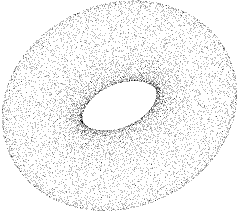
\includegraphics[width=30mm]{figures/Point_cloud_torus1.png}
	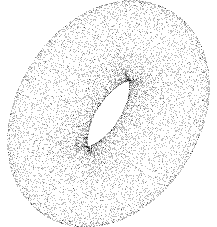
\includegraphics[width=30mm]{figures/Point_cloud_torus2.png}
	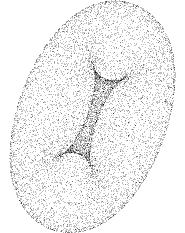
\includegraphics[width=30mm]{figures/Point_cloud_torus3.png}
	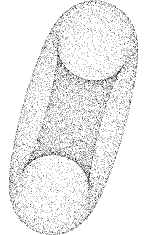
\includegraphics[width=30mm]{figures/Point_cloud_torus4.png}
	\caption{Ett komplett punktmoln som representerar ett torus objekt.}
	\label{fig:point_cloud_torus}
\end{figure}

\begin{figure}[H]
	\centering
	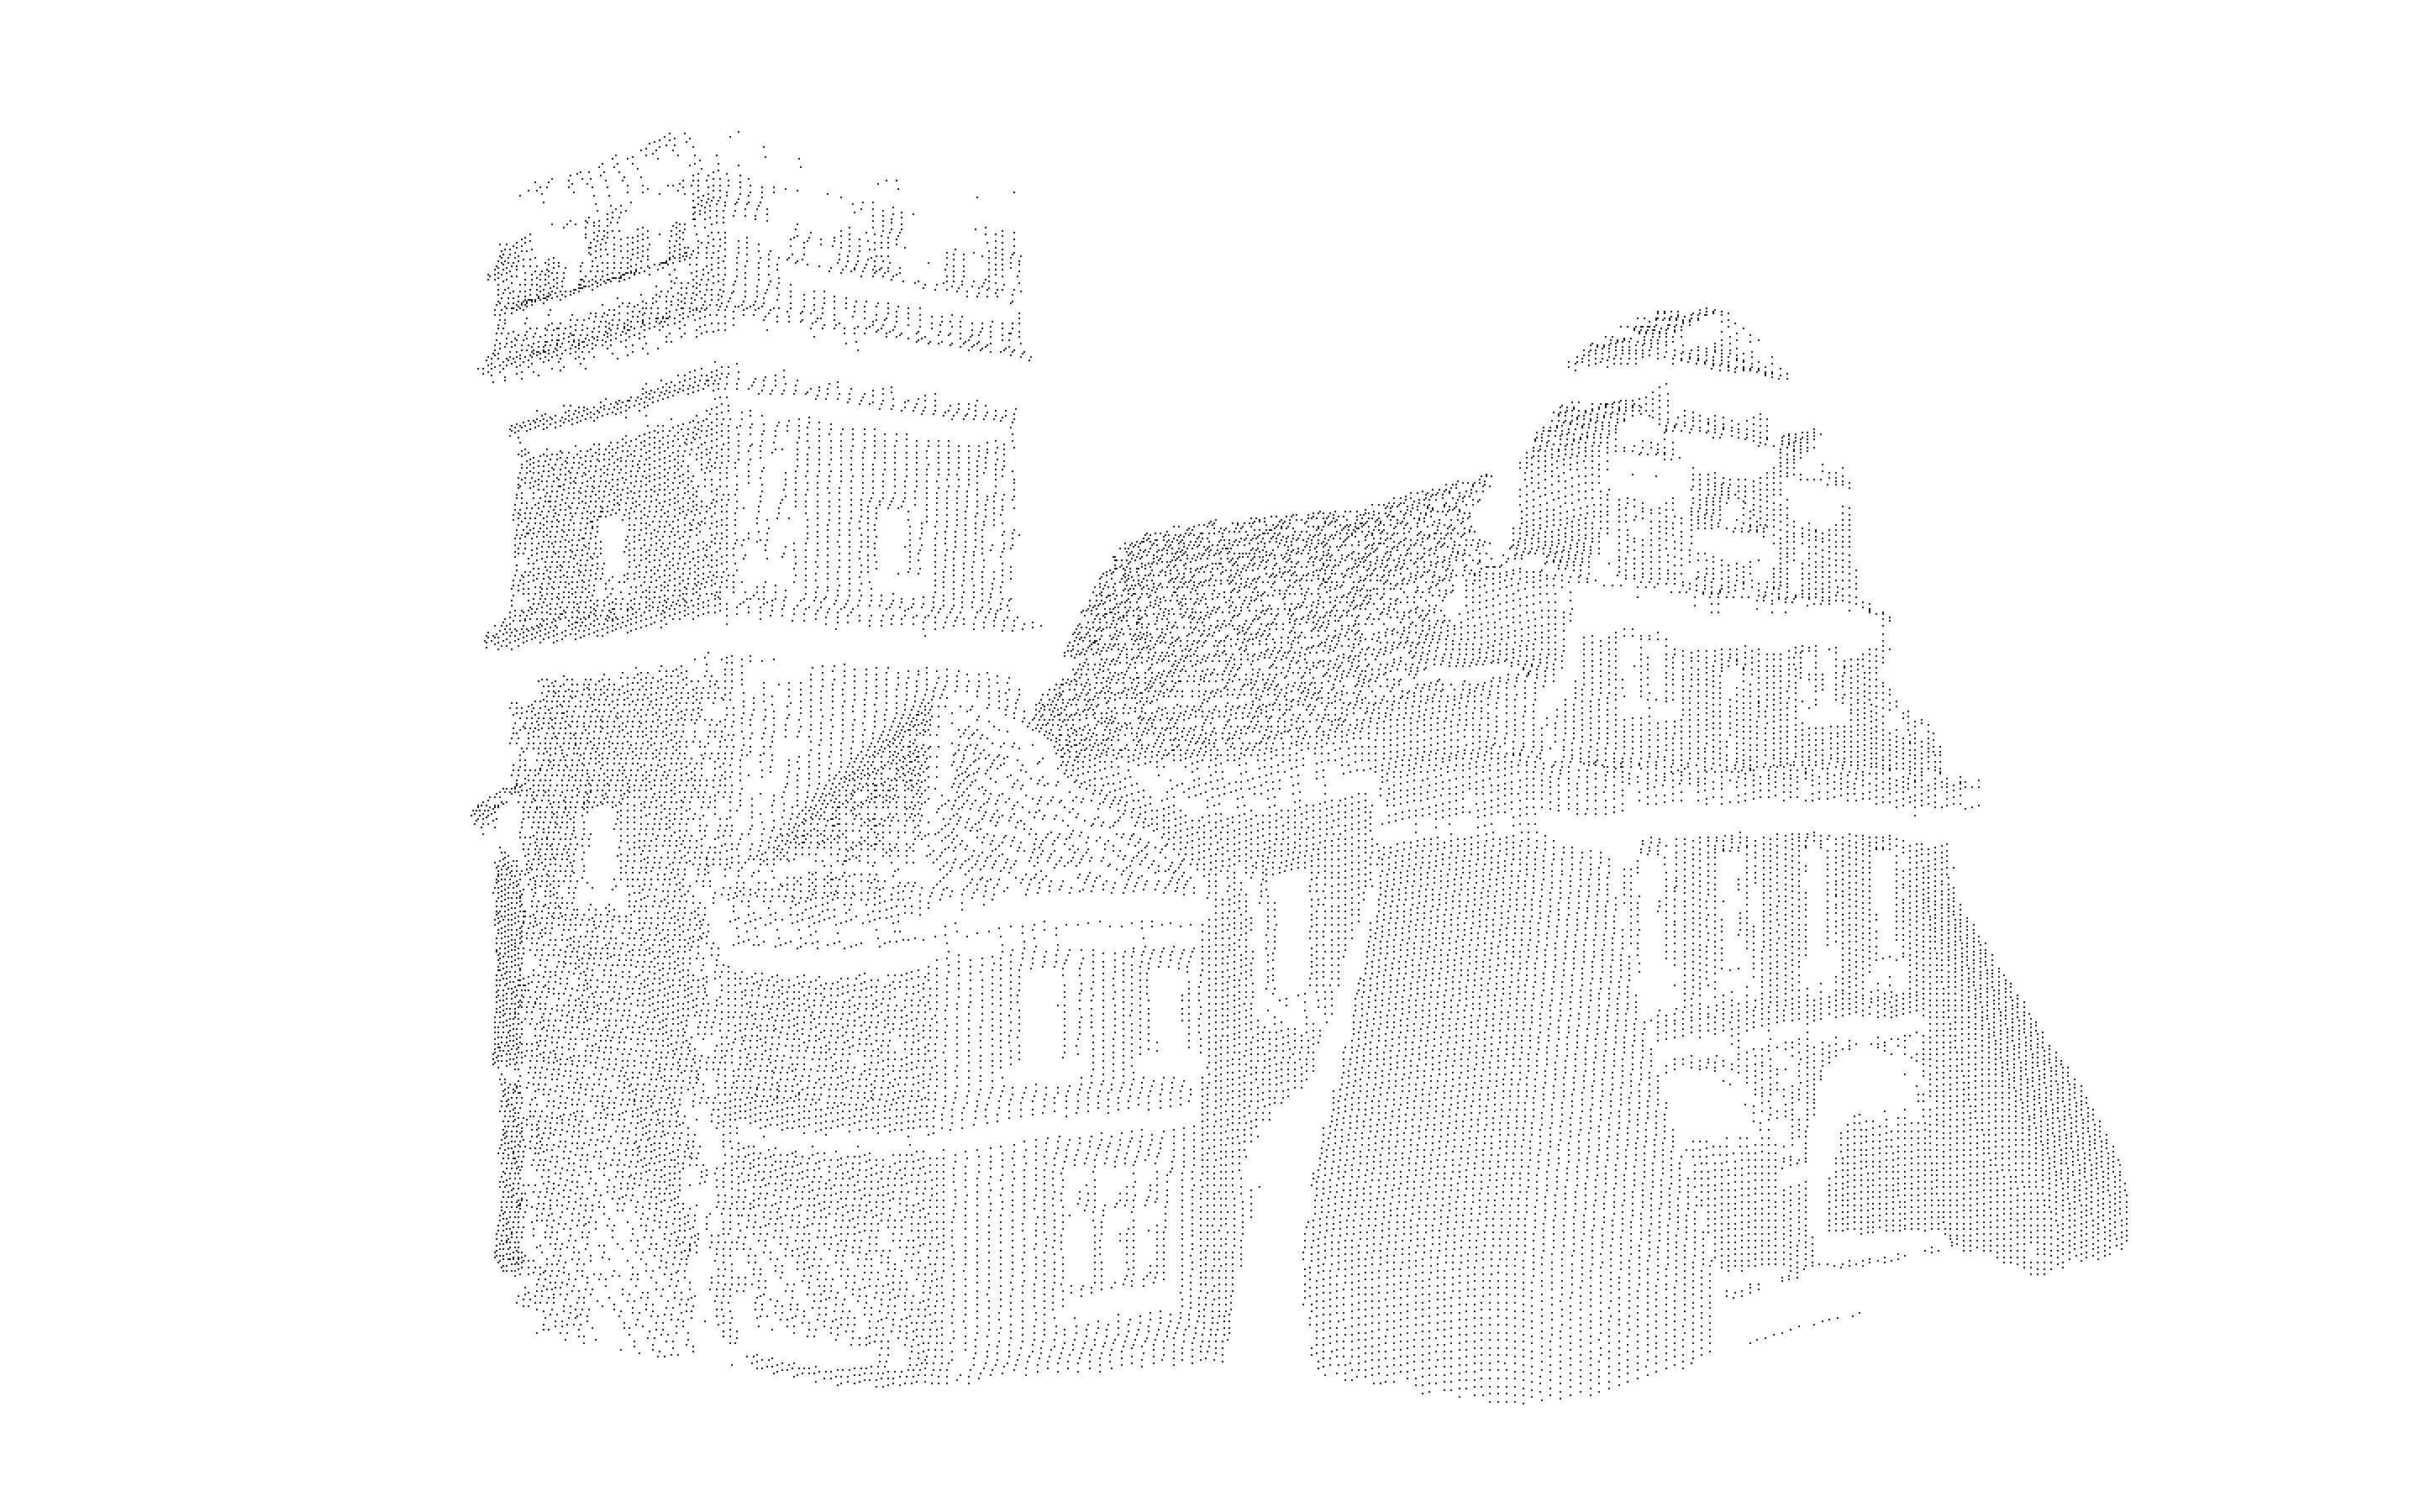
\includegraphics[width=100mm]{figures/icke_komplett_moln_kyrka.png}
	\caption{Ett icke komplett punktmoln som representerar en del av en kyrka.}
	\label{fig:point_cloud_church}
\end{figure}

\section{Point Cloud Library}

Point Cloud Library (PCL) är ett bibliotek till C++ som bidrar med algoritmer till att behandla 3D-objekt. PCL innehåller bland annat algoritmer för:

\begin{itemize}
	\item filtrering
	\item registrering
	\item segmentering
	\item modellanpassning
	\item ytrekonstruering
	\item funktionsestimering.
\end{itemize}
PCL är alltså ett bibliotek avsett att ge stöd till att behandla punktmolnsdata, i form av olika bearbetningsalgoritmer \cite{rusu20113d}.

PCL använder sig av ett eget visualiseringsbibliotek för att visualisera punktmoln. Visualiseringsbiblioteket i PCL integrerar med visualiseringsverktyget VTK \cite{VTK_book}\cite{rusu20113d}.

Nedan beskrivs de olika algoritmerna som PCL innehåller. De algoritmer som beskrivs är de algoritmer som är relevanta för detta projekt.

\subsection{Filtrering}
PCLs filtreringsbibliotek innehåller algoritmer för att filtrera bort skräppunkter från ett punktmoln. Dessa skräppunkter kan uppstå vid skanning av ett objekt eftersom avståndskameran kan reagera på bakgrunden och inte bara på objektet. Det gör att skräppunkter infaller i punkmolnet. För att kunna behandla punktmolnet måste dessa skräppunkter först filtreras bort.

PCL har stöd för flera olika metoder för filtrering. Första steget i vår filtrering är att ta bort alla punkter som ligger utanför ett visst intervall av koordinater. Syftet med detta är att ta bort sådant som måste ligga utanför det skannade objektet. I nästa steg kontrolleras det för varje punkt hur många grannar den punkten har inom en viss radie. Alla punkter som har under ett visst antal grannar tas bort vilket leder till att enstaka punkter som inte ligger i närheten av något objekt tas bort \cite{pcl_filtering}.

För att undvika att punktmoln blir för stora, det vill säga får för många punkter så att de tar för lång tid att behandla, kan nedsampling (från eng. \textit{"down sampling"}) användas för att ta bort punkter och samtidigt uppskatta den yta som representeras så nära som möjligt. För att göra detta i PCL delas punktmolnet som ska nedsamplas in i voxels, vilket kan ses som att punktmolnet delas in i ett antal kuber. Sedan ersätts alla punkter i varje kub med en punkt som ligger i centrum för alla punkterna i kuben. På detta sätt ges en nära uppskattning av den representerade ytan med mycket färre punkter än det ursprungliga punktmolnet \cite{voxel_grid}.
 

\subsection{Registrering}
Att kombinera två punktmoln till ett punktmoln som innehåller samma information kallas för att "registrera punktmoln". Detta är en komplicerad process där både translationen och rotationen, runt alla axlar, kan behöva ändras. Målet med parvis registrering, registrering av två punktmoln, är att flytta ett moln så att alla punkter som överlappar i de två separata molnet överlappar i resultatmolnet. I PCL finns ett registreringsbibliotek som innehåller algoritmer för registrering\cite{pcl_registration}. För mer information angående registreringen och dess algoritmer, se Michaels Karlssons individuella utredning i kapitel \ref{cha:indiv-report-karlsson}.  

%Att anpassa olika punkter i ett punktmoln så att de representerar en komplett modell över objektet kallas för punktmolnsregistrering. Registrering är ett stort problem och PCL erbjuder ett registreringsbibliotek för ändamålet. Målet med registreringen är att hitta de relativa positionerna och orienteringarna för de separata punktmolnen (tagna från olika vyer) så att varje punkt i respektive moln överlappar perfekt med varandra \cite{pcl_registration}. För mer information angående registreringen och dess algoritmer, se Michaels Karlssons individuella utredning i kapitel \ref{cha:indiv-report-karlsson}.

För att registrera punktmoln finns ett antal olika algoritmer med olika för- och nackdelar. En vanlig algoritm är \textit{Iterative Closest Point} (ICP). Det är en så kallad parvis registreringsalgoritm som registrerar enbart ett punktmoln till ett annat. ICP går ut på att minimera summan av avståndet från varje punkt i det ena punktmolnet till varje punkt i det andra punktmolnet.

För att begränsa antalet punkter som måste beräknas används parametern \textit{Max correspondence distance} så att enbart de punkter inom avståndet räknas in i summan för varje punkt. \textit{Transformation epsilon} är ett mått på hur mycket transformationen för punktmolnet som ska matchas in får ändras för varje iteration. Genom att öka detta epsilon kan, vid behov, algoritmen flytta punktmolnet längre och därmed nå sitt mål på färre iterationer. Nackdelen med ett för högt epsilon är dock att punktmolnet kan flyttas förbi optimum som därmed slösar tid. Slutligen kan \textit{Max iterations} användas för att avgöra hur många gånger algoritmen ska köras för varje parvis registrering. Genom att öka antalet iterationer ökar tidsåtgången men resultatet förbättras också.

\subsection{Ytrekonstruering}
PCLs ytrekonstrueringsbibliotek innehåller algoritmer för att rekonstruera de ursprungliga ytorna från 3D-skanningar. Beroende på uppgiften kan PCL till exempel rekonstruera en ojämn yta till en jämn, en meshrepresentation av ett komplett punktmoln eller en yta med normaler \cite{pcl_surface_reconstruction}.

Att rekonstruera en ojämn yta till en jämn kan vara viktigt om molnet är brusigt, eller om det består av flera skanningar som inte är perfekt anpassade. PCLs ytrekonstrueringsbibliotek kan även skapa en konkav modell av ett punktmoln. Detta kan vara bra om till exempel gränserna i ett punktmoln behöver extraheras \cite{pcl_surface_reconstruction}.

Meshning av ett punktmoln görs efter att punktmolnen registrerats så de bildar ett komplett punktmoln. Att skapa en meshrepresentation av ett komplett punktmoln innebär att skapa en yta utan punkter. Meshrepresentationen av punktmolnet är alltså en vattentät 3D-modell uppbyggd av polygoner. Den algoritm som används för att mesha ett punktmoln i detta projekt är en trianguleringsalgoritm (Poisson surface reconstruction) som körs på ett punktmoln med normaler för att erhålla en yta baserad på grannarna till respektive punkt. För detta krävs alltså ett punktmolnsobjekt som innehåller normalerna till varje punkt i punktmolnet. I detta punktmoln med normaler kan sedan önskade parametrar sättas innan själva trianguleringsalgoritmen körs för att generera den önskade meshen \cite{pcl_surface_reconstruction}\cite{pcl_triangulation_algorithm}. 


\section{3D-skrivare}
En 3D-skrivare kan användas för att skriva ut 3D-objekt i plast utifrån modeller i en dator. För att kunna göra detta har skrivaren ett styrkort som exekverar så kallad G-code \cite{gcode}. Denna G-code beskriver vilka motorer som ska flyttas och hur mycket. En 3D-modell som är sparad i datorn, i form av en mesh, måste alltså behandlas genom att använda en algoritm för att generera G-code utifrån modellen. Detta görs ofta genom en typ av programvara som kallas för slicer. Namnet kommer av att programmet delar upp modellen i olika lager och sedan genererar hur skrivaren måste röra för att skriva ut ett lager. På detta sätt byggs sedan hela den ursprungliga modellen upp lager för lager. Två vanliga slicer-programvaror är \textit{Cura} \cite{cura} och \textit{Slic3r} \cite{slic3r}.

\section{Systemanatomi}
En systemanatomi, vars viktigaste egenskap är enkelheten, är en visuell beskrivning av ett system som gör det enkelt för samtliga i utvecklingsgruppen att förstå systemet och dess interna beroenden. Systemanatomin är särskilt användbar vid utveckling av stora komplexa system i agila utvecklingsgrupper eftersom det ger en gemensam syn över systemet. En systemanatomi säger inget om hur systemet ska implementeras eller hur det är uppbyggt rent tekniskt utan det enda den säger är vilken funktionalitet systemet ska innehålla och vad systemet ska kunna utföra. Därför kan en systemanatomi inte ersätta andra modeller eller designverktyg utan det är enbart ett annat sätt att beskriva systemet och vad det ska göra \cite{system_anatomy}.


\section{Hållbar utveckling}
Hållbar utveckling är en relevant aspekt i dagens utveckling av programvaror eftersom de används kontinuerligt av samhället. Effekterna som en programvara bidrar med i samhället beror på hur den har producerats och hur den används av konsumenterna. Detta gör att effekterna som en programvara bidrar med i samhället kan vara både positiva men också djupt negativa \cite{raturi2014developing}. Hållbarhet definieras som "förmåga att uthärda" och "bevara funktionen hos ett system under en utsträckt tidsperiod". Att analysera hållbarhet hos ett mjukvarusystem innebär för de som utvecklar systemet att ha dessa fyra områden i åtanke \cite{lago2015framing}:

\begin{itemize}
	\item Ekonomiskt -  Systemet ska bevara kapital och värde.
	\item Socialt - Systemet ska underhålla samhället.
	\item Miljö - Systemet ska skydda den mänskliga välfärden genom att skydda naturens tillgångar.
	\item Tekniskt - Systemet ska utvecklas för att stödja långtidsanvändning.
\end{itemize}
En mer ingående beskrivning om hur vårt projekt främjar hållbar utveckling diskuteras i avsnitt \ref{disc:hållbar_utveckling}.


%%%%%%%%%%%%%%%%%%%%%%%%%%%%%%%%%%%%%%%%%%%%%%%%%%%%%%%%%%%%%%%%%%%%%%
%%% theory.tex ends here

%% 
\chapter{Metod}
\label{cha:method}

\section{Utvecklingsmetodik}

I projektet har en iterativ process använts med vissa inslag av vattenfallsmodellen. Utvecklingsledaren ansvarade för att ta fram vad som skulle genomföras i varje iteration och planera iterationerna i samråd med övriga gruppmedlemmar. Teamledaren ansvarade för att planera de administrativa delarna av projektet. För att planera en iteration utgick gruppen från kravspecifikationen och bröt ner den till aktiviteter. Målet med varje aktivitet var att den skulle vara genomförbar på mindre än en vecka. När aktiviteterna var skapade gjorde utvecklingsledaren med inrådan från bland annat arkitekten en tidsuppskattning på varje aktivitet och hur många som borde jobba med aktiviteten. Efter planeringen gick gruppen igenom aktiviteterna för att alla i gruppen skulle bli informerade om vad som skulle genomföras under iterationen. När alla i gruppen var informerade om aktiviteterna valde gruppmedlemmarna vilka aktiviteter som de ville delta i. Vidare under iterationen planerades hur aktiviteten skulle utföras av de gruppmedlemmar som valt den aktiviteten.

\subsection{Förstudie}

Projektet inleddes med en förstudiefas där gruppen sammanställde diverse dokument. Syftet med dessa dokument var att både gruppmedlemmarna själva och externa parter skulle få en bättre insikt i vad projektet gick ut på och vad dess mål var. Dokumenten utformades och togs fram av den eller de personer i gruppen som var bäst lämpade för ett visst dokument. Med det menas den person som passade bäst för ett visst dokument med avseende på dennes roll i gruppen.

Gruppen började sedan att studera de områden, verktyg och ramverk som skulle behövas för projektet. Den information som gruppen hade från början var den som kunden tillhandahållit och utifrån denna information upptäcktes en del nya områden som behövde undersökas, framförallt PCL. Under förstudien delade utvecklingsledaren ut olika områden att undersöka. Efter ett område undersökts skrevs ett kort dokument som beskrev slutsatserna och innehöll relevanta länkar från undersökningen. De största områdena som undersöktes var ROS och PCL. Framförallt undersöktes ROS eftersom det hade en stor påverkan på hur arkitekturen och implementation skulle genomföras. Att undersöka ROS noggrant var dessutom viktigt då tidigare erfarenhet inom ROS saknades hos samtliga gruppmedlemmar. 
Undersökningarna inom ROS avslutades först med att alla i gruppen genomförde de guider som rekommenderades på ROS hemsida. Efter att guiderna var genomförda skrev alla gruppmedlemmar varsin chattklient med hjälp av ROS.

\subsection{Iteration 1}

Iteration 1 omfattar de två första veckorna efter förstudiefasen. Huvudmålet för iteration 1 var att få klart basfunktionaliteten för produkten. Under första veckan låg fokus på att skriva kod, skapa ett gränssnitt till den existerande mjukvaran, samt att registrera och mesha punktmoln. Under andra veckan flyttades fokus till att färdigställa den dokumentation som skulle lämnas in efter iteration 1, samt att färdigställa så mycket som möjligt av det som påbörjades under första veckan.

\subsection{Iteration 2}

Iterationen inleddes med fokus på registrering då detta var det stora frågetecknet i projektet vid början av iteration 2. Efter att först ha undersökt olika algoritmer beslutades det att gruppen skulle fortsätta med ICP då den hade bäst stöd i PCL-biblioteket. Efter det delades gruppen i två för att arbeta med två olika algoritmer för att registrera punktmoln. Den första algoritmen var att försöka vrida och placera punktmolnen rätt från början och på så sätt få det enklare att sedan registrera punktmolnen med ICP. Vrida och placera punktmolnen rätt innebär att först rotera dem så att de har rätt rotation i förhållande till varandra och sedan sätta origo till samma punkt för alla punktmolnen. Problemet med att få algoritmen att fungera var att den behövde vara väldigt generell vilket gjorde den svår att ta fram och fullända. Speciellt för de objekt som i början av projektet ansågs enkla att registrera av gruppen och kunden. Ett exempel på dessa enkla objekt var släta rätblock. Den andra algoritmen var mer anpassad för de då ansedda enkla objekten. Den gick ut på att i första hand endast lösa problemet med att registrera rätblocksliknande föremål. Detta gjorde den genom att hitta den plattaste ytan, anta att det var en sida och sedan ta fyra skanningar med 90 graders rotation mellan varje. Dessa punktmoln registrerades sedan på ett genererat rätblock med ICP.

Den andra algoritmen var den som utforskades mest tills den skulle börja testas ihop med hårdvaran. Då upptäcktes att det fanns mängder med fel på det underliggande systemet som tog fram punktmolnen. Det gick inte att genomföra tillräckligt många skanningar i rad utan att det underliggande systemet kraschade.

Detta gjorde att gruppen tillsammans med kunden fick revidera en stor del av projektet där gruppen bortsåg från det tidigare systemet helt och hållet. Gruppen beslutade också tillsammans med kunden att det borde vara lättare att registrera mer detaljerade objekt. Gruppen gick då tillbaka till algoritmen för att placera rätt och sedan registrera. Denna nya registrering placerades i ett helt nytt program, 3DCopy. Gruppen började då bygga ett CLI och integrera meshning och registrering i det programmet. Istället för att som tidigare bygga allt som enskilda ROS-noder.

\subsection{Iteration 3}

Iteration 3 omfattar fyra veckor efter iteration 2. Den första veckan låg fokus på att färdigställa de individuella delarna av kandidatrapporten inför inlämning. En del arbete genomfördes också på den gemensamma rapporten som också skulle lämnas in. Rapporten lämnades sedan in i slutet av första veckan. Andra veckan låg fokus på den gemensamma delen av rapporten. En del komplettering av de individuella delarna gjordes också då gruppen fick feedback på första veckans inlämning redan i början av andra veckan i iteration 3.

Resterande två veckor arbetades det med att bryta ut registrering och meshning från ROS-systemet och integrera det med det nya programmet 3DCopy. Därefter färdigställdes 3DCopy med kommandoradsgränssnitt och grafiskt användargränssnitt. Det skrevs också mjukvara för att kunna ta fram och filtrera punktmoln från TreeDs system. Parallellt med detta genomfördes opponering samt förberedelser för redovisning av erfarenheter och slutp\-resentation.  


\section{Metod för att fånga erfarenheter}

Erfarenheter fångades upp under projektets gång med hjälp av kontinuerlig utvärdering och diskussioner under gruppens gemensamma möten. Dessa möten skedde två gånger i veckan, varje måndag och torsdag. På måndagar deltog även handledaren och då låg fokus på en statusuppdatering och vad som skulle göras i veckan. Under statusuppdateringen diskuterades vad som gått bra, vad som gått dåligt och hur gruppen skulle kunna förbättra saker och ting. Under torsdagsmöten lades fokus på diskussion kring viktiga frågor som hela gruppen behövde vara del av. Erfarenheterna som kommit upp på dessa möten, framförallt måndagsmötena sammanfattades av teamledaren i varje veckas statusrapport.

Erfarenheter har också delats av gruppen under arbetets gång. Då gruppen arbetat större delen av tiden i samma rum har det skett mycket diskussion i gruppen kring olika problem öppet i rummet. Slutligen har gruppmedlemmarna under projektets gång samlat de erfarenheter som de fått i den här rapporten. Därmed så har erfarenheter samlats in kontinuerligt under genomförandet av projektet.


%%%%%%%%%%%%%%%%%%%%%%%%%%%%%%%%%%%%%%%%%%%%%%%%%%%%%%%%%%%%%%%%%%%%%%
%%% method.tex ends here

\chapter{Resultat}
\label{cha:results}

\section{Systembeskrivning - vidareutveckling av TreeD}
\label{cha:results-systembeskrivning-treed}
%% Översiktlig beskrivning system, dokument
%% Vad har kunden för värde hos det som skapats?

Nedan följer en beskrivning av det ROS-baserade system som byggde vidare på TreeD och som utvecklades innan kraven i projektet omförhandlades med kunden.

Systemet bestod hårdvarumässigt av ett rotationsbord, en avståndskamera och en linjärenhet för att flytta avståndskameran längs en axel. För att styra detta fanns det sedan tidigare mjukvara som kan utföra en enskild skanning. Projektet skulle ha resulterat i en mjukvara för att utföra fler skanningar från olika vinklar och sammanfoga dessa till ett komplett objekt som kan skrivas ut på en 3D-skrivare.

Tidigt i arbetet togs en systemanatomi fram, se figur \ref{fig:system_anatomy}, som beskriver vilken funktionalitet systemet skulle ha. Denna hjälpte även till med att dela in närliggande funktionalitet i moduler och låg som underlag för arkitekturbeskrivningen.

\begin{figure}[H]
	\centering{\tiny }
	\includegraphics[width=130mm]{figures/system_anatomy.png}
	\caption{Översikt över systemanatomin.}
	\label{fig:system_anatomy}
\end{figure}


Arkitekturbeskrivningen som togs fram för systemet förklarar hur systemet skulle fungera och vilka moduler som skulle finnas. Arkitekturen gav en bra utgångspunkt för hur systemet skulle implementeras. I arkitekturbeskrivningen finns det förklarat vilka noder systemet skulle bestå av och hur de skulle kommunicera med varandra.

Denna arkitektur är uppbyggd i ROS vilket innebär att de flesta noder i det tänkta systemet fungerar som en service som tar emot ett anrop för att utföra någonting och när den är klar svarar den med resultatet av arbetet. Detta gör att alla noder har tydliga gränssnitt mellan varandra vilket resulterar i en bra separation mellan olika moduler.

Systemet var uppbyggt enligt en förenklad variant av \textit{pipe and filter}-modellen, där resultatet av ett steg skickas vidare som indata till nästa steg i modellen. Detta flöde styrs av klienten så att användaren kan välja att köra hela eller delar av processen. Figur \ref{fig:noddiagram} visar hur systemet var uppbyggt.

\begin{figure}[H]
	\centering
	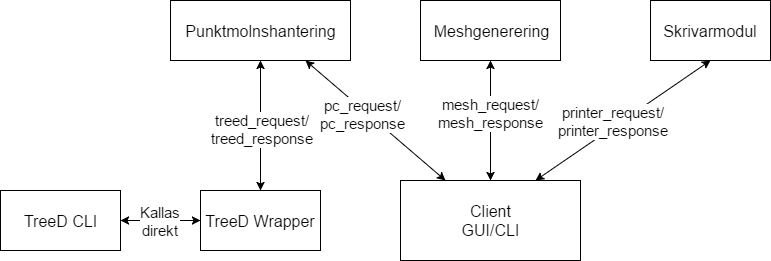
\includegraphics[width=130mm]{figures/Noddiagram.png}
	\caption{Diagram över ROS-noderna i den första versionen av systemet.}
	\label{fig:noddiagram}
\end{figure}

Det tänkta systemet kunde samla in fler punktmoln. Detta gjordes av punktmolnshanteringsnoden som tar in ett värde för hur noggrant objektet ska skannas. Punktmolnshanteringsnoden utför ett antal skanningar genom att noden TreeD-wrapper kallas. Sedan registrerar punktmolnshanteringsnoden dessa inkompletta punktmoln till ett punktmoln som representerar hela objektet.

När ett komplett punktmoln har genererats skickas det vidare till meshgenereringsnoden som uppskattar en tredimensionell yta, även kallad mesh, bestående av polygoner utifrån punktmolnet. Denna mesh kan sedan användas för att generera kod som kan köras på en 3D-skrivare för att skriva ut objektet.

Mycket tid under de första iterationerna av projektet spenderades på att utforska och undersöka olika tekniker och algoritmer. Som resultat av det finns det mycket nyttig kunskap i projektgruppen och även en del testkod för att utföra olika delar.

Det ROS-baserade systemet var uppdelat i en serverdel och en klient. Tanken var att servern skulle köras på en dator som var fysiskt kopplad till hårdvaran och på så sätt kunde styra den genom TreeD-wrappern. Klienten skulle i första hand köras på samma dator och styra servern men med möjligheten att köras på en annan dator och styra servern över nätverket. Se figur \ref{fig:systembeskrivning_gamla} för en bild på hur det tänkta systemet var planerat att vara strukturerat.

\begin{figure}[H]
	\centering
	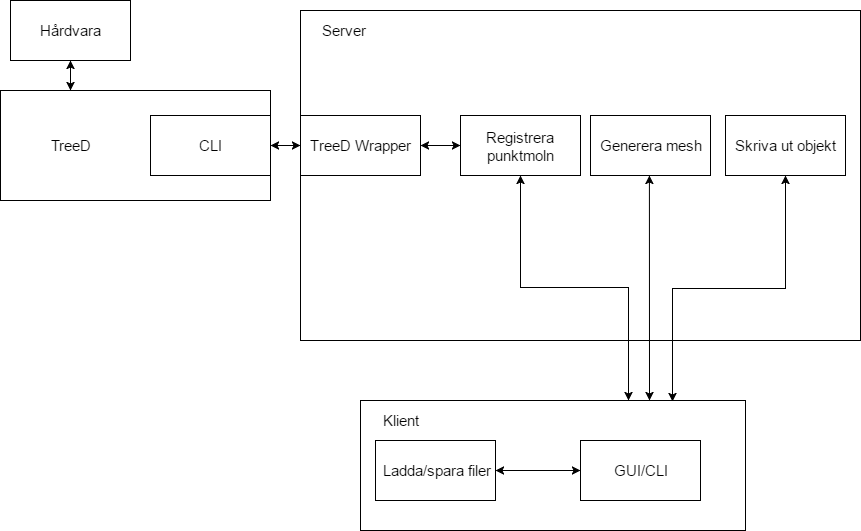
\includegraphics[width=130mm]{figures/Systemskiss_gamla.png}
	\caption{En skiss av det tänkta ROS-baserade systemet.}
	\label{fig:systembeskrivning_gamla}
\end{figure}

Som kan ses i figurerna \ref{fig:noddiagram} och \ref{fig:systembeskrivning_gamla} så är klienten den centrala delen i programmet. Den hanterar användarens indata och använder sig av de olika noderna för att utföra det användaren vill. Konceptet var att systemet skulle använda en \textit{pipe and filter}-arkitektur. Där klienten skickade runt data i pipen men att användaren, genom klienten hade möjlighet att granska resultatet och göra viss handpåläggning mellan de olika stegen. Detta genom att klienten alltid kan spara resultatet från ett steg till fil och använda andra program för handpåläggningen innan den skickas vidare i systemet.

\section{Systembeskrivning - 3DCopy}

Som kan läsas tidigare i denna rapport så omförhandlades projektets krav och mål med kunden under projektets gång. Detta ledde till att gruppen gjorde om systemets arkitektur. ROS-arkitekturen som presenterats i avsnitt 5.1 byttes ut mot att istället skapa ett objektorienterat program, skrivet i C++. Detta program utför både registrering, filtrering och meshning. När sedan den meshen genererats kan programmet skriva ut objektet med hjälp av en 3D-skrivare. Till detta program finns också ett CLI och ett GUI.

\subsection{Arkitektur}
Programmet består av två större klasser, \textit{Registration} och \textit{Mesh}. Dessa två klasser används sedan av antingen \textit{Cli}  eller \textit{Gui} klasserna, vilket visas i figur \ref{fig:class_diagram}.  Det har lagts stor vikt vid moduläriteten i programmet då \textit{Registration} och \textit{Mesh} ska fungera självständigt i olika program.

\begin{figure}[H]
	\centering
	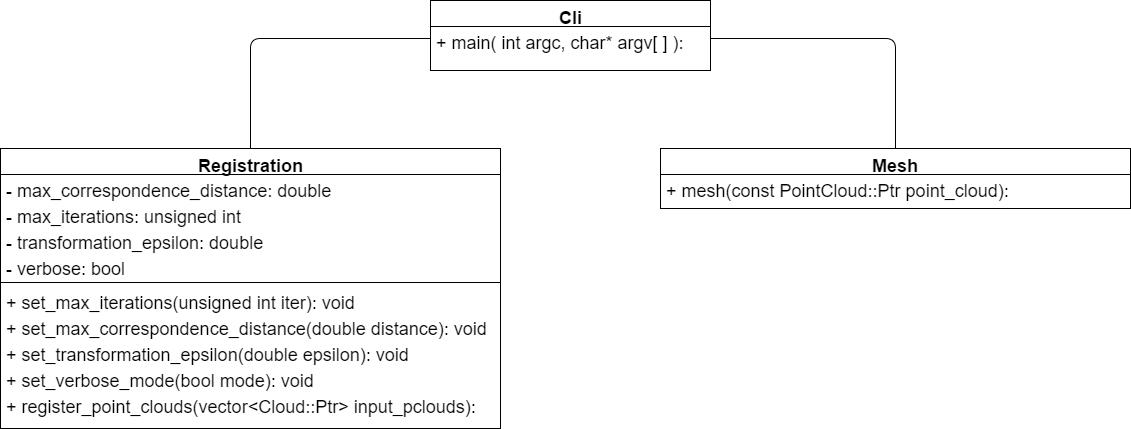
\includegraphics[width=130mm]{figures/klassdiagram.png}
	\caption{Översiktligt klassdiagram över arkitekturen}
	\label{fig:class_diagram}
\end{figure}

\subsection{Kommandoradsgränssnitt (CLI)}

Systemet kan kontrolleras av ett CLI som kan ta in olika parametrar för att anpassa registreringen. Det finns även alternativ för att bara registrera eller bara mesha objekt. När man kör programmet med hjälp av kommandoradsgränssnittet väljer man vilka filer eller mappar med filer programmet ska läsa in och använda. Hur de används beror på alternativen. Ett exempel på ett anrop är:\\\\
\texttt{3DCopy -v --max-corr-dist 15 path/to/register/ output}\\\\
Det anropet kommer registrera och sedan mesha pcd-filerna i mappen \textit{path/to/register/} och döpa det kompletta punktmolnet respektive färdiga meshen till \textit{output.pcd} och \textit{output.stl}. Under registreringen och meshningen kommer programmet att skriva ut information om processen på grund av \texttt{-v} flaggan som står för \textit{verbose mode}. Om man undrar vilka alternativ som finns kan man använda \texttt{-h} flaggan så skriver programmet ut det samt hur man använder programmet med hjälp av kommandoradsgränssnittet. 

\subsection{Grafiskt användargränssnitt (GUI)}
För att lättare kunna styra systemet utvecklades också ett GUI. GUI:t har nästintill samma funktionalitet som CLI:t och målet med att ha samma funktionalitet är att det inte ska spela någon roll om man använder CLI eller GUI.

\begin{figure}[H]
	\centering
	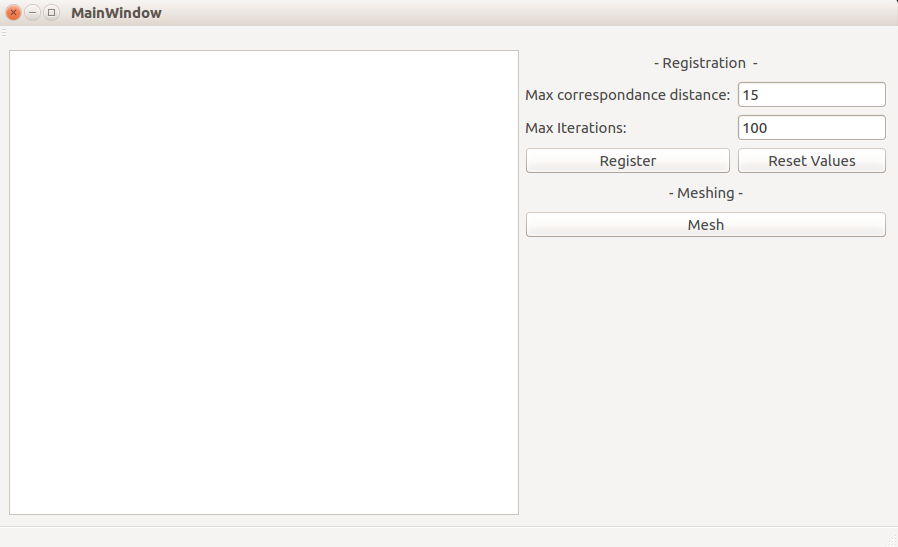
\includegraphics[width=130mm]{figures/3DCopyGUI.PNG}
	\caption{GUI:t för 3DCopy.}
	\label{fig:3dcopy_gui_res}
\end{figure}

De funktioner som finns i GUI:t är \textit{Register} som öppnar en dialog där man får välja en mapp som innehåller de punktmoln som man vill registrera. Det finns också en \textit{Mesh}-funktion där en dialog öppnas och man får välja det punktmoln som man vill mesha. Slutligen finns det en funktion för att återställa parametervärdena för registreringen, \textit{Reset Values}. De värden som återställs är \textit{Max correspondence distance} och \textit{Max iterations} till 15 respektive 100.

\subsection{Registrering}
Systemet registrerar punktmoln parvis genom att använda PCLs implementation av ICP. De punktmoln som läses in i antingen CLI:t eller GUI:t behandlas av registreringsklassen och utför registreringen. För att registreringen ska fungera för olika fall kan användaren själv sätta värden på parametrarna \textit{Max correspondence distance}, \textit{Transformation epsilon} och \textit{Max iterations}.

\subsection{Meshning}
Den ytrekonstruering som systemet använder, PCLs \textit{Poisson surface reconstruction}, är väldigt beroende av att det registrerade punktmolnet inte har några punkter som har hamnat fel. Om några punkter är fel eller om det är för glest mellan punkterna så kan inte algoritmen räkna ut ytnormalerna korrekt. Om ytnormalerna blir fel kommer inte meshen att stämma överens med det objekt som punktmolnet föreställer.

\begin{figure}[H]
	\centering
	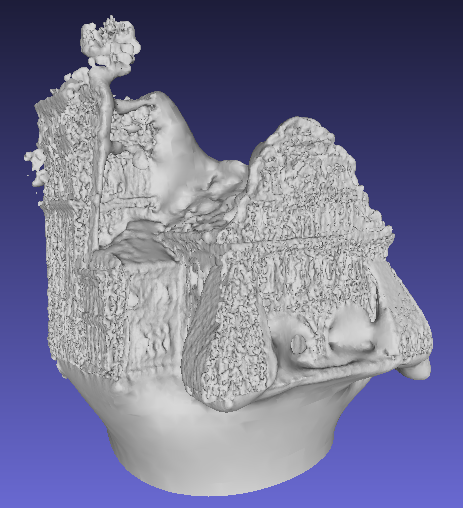
\includegraphics[width=80mm]{figures/3DCopyMeshChurch.PNG}
	\caption{Mesh av icke komplett punktmoln som föreställer en kyrka.}
	\label{fig:3dcopy_mesh_church}
\end{figure}
\label{cha:results_experiences}

I figur \ref{fig:3dcopy_mesh_church} kan man se var de olika problemen uppstår. Ovanpå och undertill kyrkan kan man se att det saknas punkter där det blir släta, rundade ytor som inte följer kanterna. Det syns också tydligt på flera ställen där meshen blir grynig att punkterna inte har hamnat rätt.

\section{Gemensamma erfarenheter}
%% Goda, mindre bra
%% I projektets alla faser
%% Tekniska, process-relaterade

I detta avsnitt presenteras de erfarenheter som gruppen har samlat på sig under projektets gång.

\subsection{Övergripande projekterfarenheter}

Att göra efterforskningar innan man börjar med någonting är väldigt viktigt och det märktes direkt i projektets början. Både genom att större delen av våra efterforskningar kom till stor hjälp direkt i projektet och bara några dagar in i första iterationen märktes det att det fanns några områden vi behövde läsa på mer om innan vi kunde skriva kod. Ett exempel på bra efterforskning som gjordes i förstudien var efterforskningarna kring ROS där alla gruppmedlemmar gick igenom handledningsexempel och läste dokumentation som utvecklingsledaren gått igenom och tagit fram. I slutet av förstudien gjordes en gemensam kodutmaning där alla fick skriva varsin chattklient med hjälp av ROS. Kodutmaningen ledde till att alla kom in i ROS, Git, Python och andra verktyg som skulle användas under resten av projektet.


\subsection{Erfarenheter gällande kommunikation}

Betydelsen av kommunikation var stor under projektets gång. Verktygen \textit{Slack} och \textit{Trello} har använts flitigt och varit givande för gruppen. Med \textit{Slack} har vi alltid kunnat nå varandra snabbt och smidigt. Vi har kunnat hålla informationsflöden skilda och sorterade i olika kanaler. Funktioner som påminnelser och trådar har också varit till stor hjälp för att lätt kunna komma åt den informationen som man vill åt i flödena.

För att ha en översikt i hur det går med olika delar av projektet har gruppen använt \textit{Trello}. Genom att ha olika listor för statusen av dokument och funktioner under utveckling har gjort att man som gruppmedlem lätt kunnat se hur det går och vad man behöver göra.


\subsection{Erfarenheter gällande kvalité}

Kvalité har varit viktigt för gruppen och kvalitetsansvarig har gjort ett bra jobb med att se till att projektets kod och dokument håller en hög standard. Detta framförallt genom granskning av dokument och kod. All kod i projektet har genomgått granskning för att säkerställa god kvalité. Till detta har Githubs pull request-funktion använts där alla gruppmedlemmar kunnat kommentera och diskutera koden innan den går in i master branchen på repositoriet. Dokumenten har också granskats, då genom korrekturläsning. All denna granskning har varit mycket bra för att se hur andra skriver dokument och kod.


\subsection{Erfarenheter av att bygga vidare på ett projekt}

I mitten av projektet upptäckte gruppen att det system som skulle vidareutvecklas inte fungerade tillräckligt stabilt för att det skulle vara möjligt att integrera med det system som gruppen utvecklade. Gruppen litade på att kunden hade god insikt i det tidigare systemet och eftersom att dessa fel inte togs upp i början av projektet förutsatte gruppen att det tidigare systemet inte innehöll några fel.

Eftersom att gruppen inte hade någon anledning att tro att det tidigare systemet innehöll fel så genomfördes ingen rigorös testning av det tidigare systemet. Det saknades också testdokumentation och  annan dokumentation från den grupp som hade utvecklat det tidigare systemet. Det visar vikten av att väl dokumentera sitt system för att undvika problem i framtiden.


\section{Översikt över individuella bidrag}

Här listas de individuella bidrag som gruppens medlemmar har bidragit med till rapporten:

\begin{itemize}
	\item Dunström, Hampus - Hur påverkas ett team av sin arbetsmiljö?
	\item Holmberg, Olof - Kontexters påverkan vid testning av GUI
	\item Jannering, Gustav - Hur kravhanteringsmetoder påverkar ett utvecklingsprojekt
	\item Karlsson, Michael - Analys av punktmolnsregistrering
	\item Lundberg, Martin - Att bygga ett system i ROS
	\item Tuhkala, Hannes - Verktyg som är lämpliga för att skriva stora dokument
	\item Wallström, Fredrik - Kvalitetsarbete i praktiken
\end{itemize}


%%%%%%%%%%%%%%%%%%%%%%%%%%%%%%%%%%%%%%%%%%%%%%%%%%%%%%%%%%%%%%%%%%%%%%
%%% results.tex ends here
\chapter{Diskussion}
\label{cha:discussion}

\section{Resultat}
\label{sec:discussion-results}

% Finns det något i resultaten som sticker ut och behöver analyseras och kommenteras?
% Hur relaterar resultaten till det material som presenteras i teorikapitlet?
% Vad betyder teorin om betydelsen av resultaten, till exempel, vad betyder det att ett visst system har ett visst numeriskt värde i en användbarhetsbedömning, hur bra eller dåligt är det?
% Finns det något i resultaten som är oväntat baserat på litteraturgranskningen, eller är allt som man teoretisk skulle förvänta sig?
\subsection{Vad återstår?}
Vad återstår för att kunden skall få ut fullt värde av produkten? Det är en definitionsfråga. Om man definierar "fullt värde för kunden" som det värde som kunden förväntade sig innan projektet eller i projektets tidiga skede så krävs minst ett nytt projekt, vars mål är att lösa problemen med TreeD och sen rekonstruera produkten från detta projekt så att den fungerar som den skulle innan omförhandlingen av kraven. Om man istället definierar "fullt värde för kunden" som det värde som kunden förväntar sig efter omförhandlingen av kraven så skulle vi hävda att väldigt lite återstår. Meshgenereringen blev inte så automatiserad som vi hade hoppats och kunden förväntat sig, men detta beror mest på svårigheter att implementera en sådan process helt automatiskt då fler olika fall kan uppstå. Målet med projektet var att använda existerande algoritmer, inte skapa nya, eftersom detta hade tagit mycket längre tid och krävt helt andra kunskaper. Utöver detta så tycker vi att kunden har fått ut det värde som kan förväntas av projektet efter omförhandlingen av kraven. 

\subsection{Tidigare projekt}
Något som gruppen har tagit med sig från de tidigare projekt gruppmedlemmarna har genomfört är tydlig struktur på interna dokument samt gruppkontrakt. Strukturen på dokumenten har hjälpt till att hålla en hög standard även på interna dokument, det vill säga dokument som enbart är till för gruppen själva. Gruppkontraktet var uppskattat i tidigare projekt och ger tydliga riktlinjer för bland annat vad som förväntas av gruppens medlemmar, hur konflikter ska lösas och hur gruppen ska arbeta för att nå projektmålet.

Något som förbättrades från tidigare projekt är kommunikationen. Under vissa projekt som gruppens medlemmar tidigare genomfört så har kommunikationen ibland varit bristande. Det har ibland varit svårt att få tag i medlemmar eller svårt att få en överblick av kommunikationen då många olika kommunikationskanaler använts. Projektgruppen löste det snabbt genom att använda slack för all kommunikation inom gruppen och delade upp kommunikationen i olika kanaler beroende på ämne. Gruppen såg också till att allas telefonnummer fanns tillgängliga ifall man behövde kontakta någon omedelbart.

\subsection{Alternativa implementationssätt}
Då projektets krav behövde omförhandlas långt in i projektet togs två olika system fram. Det första systemet som togs fram var byggt på ROS och hade en tät koppling till det tidigare systemet även om det skulle kunna användas fristående med annan hårdvara. Det andra systemet var inte lika beroende på hårdvaran som det första utan läser istället in punktmoln från filer på datorn. Det är inte heller byggt på ROS utan är implementerat helt med hjälp av klasser i C++. Båda de implementerade systemen uppfyller i princip samma systemanatomi, se fig. \ref{fig:system_anatomy}, med den enda skillnaden att det andra systemet inte kan skanna 3D-objekt utan endast läsa in punktmoln från filer.

För att registrera punktmoln finns det många algoritmer och sätt att implementera dessa. I slutändan använde vi oss av ICP då den gav bäst resultat och har bra stöd i PCL. Det finns dock fler alternativ som exempelvis JR-MPC. Detta utforskas mer i Michael Karlssons individuella utredning, se avsnitt \ref{cha:indiv-report-karlsson}.

Även för meshgenerering finns fler alternativa metoder. I vårt system används algoritmen Poisson surface reconstruction då det är en vanlig algoritm som fungerar bra i många fall. Även den har bra stöd i PCL. På den här punkten skulle en hel del kunna förbättras, antingen genom att använda andra algoritmer eller genom att implementera användandet av algoritmen bättre, exempelvis genom att justera de parametrar som sätts.

\section{Metod}
\label{sec:discussion-method}
Som kan tydligt ses i denna rapport har inte detta projekt varit perfekt. Skulden för detta ligger dels på oss (projektgruppen). Vi har under projektets gång (speciellt under projektets andra halva) varit kritiska över hur vi gått tillväga. I \ref{cha:results_experiences} har vi listat de erfarenheter som vi kunnat dokumenterats under projektets gång. Bland dessa finns erfarenheter om vad vi borde ha gjort annorlunda Vi borde ha testat det befintliga systemet mer rigoröst tidigt. Vi borde ha ifrågasatt kundens kunskap om systemet. Men vi tycker också att en del av skulden bör ligga på kunden. Vi antog att kunden, innan de utlyste ett projekt för att vidareutveckla systemet, hade testat systemet och visste dess begränsningar.

När det gäller metoden som vi använt i projektet så anser vi att själva kärnan, eller idén bakom metoden har varit bra men att några av detaljerna av implementationen av denna metod har varit mindre bra. Som grupp håller alla med att vi borde fokuserat mycket mindre på ROS i början av projektet. Vi tycker att tanken var väldigt bra, att alla gjorde tutorials och en kodutmaning tillsammans stärkte gruppens sammanhållning och skapade en bra anda i gruppen. Men vi borde ha fokuserat på t.ex. PCL eller registrering av punktmoln istället för ROS eftersom systemet, både innan och efter omförhandlingen, inte var så beroende av ROS som vi trodde att det skulle vara. Efter förstudiefasen och iteration 1 så började fler och fler problem uppstå med projektet. De flesta av dessa problem hade sin grund i det befintliga systemet. Detta gjorde att vi mindre och mindre höll fast vid den metod vi använt tidigare och gruppens sammanhållning blev sämre.      
% Diskutera och kritisera den tillämpande metoden.
% En studie är sällan perfekt. Det finns nästan alltid saker man kunde ha gjort annorlunda om studien upprepas eller med andra resurser.
% Gå igenom de viktigaste begränsningarna med din metod och diskutera potentiella konsekvenser för resultaten, anslut tillbaka till metoden samt teorin som presenteras vid behov.

% Diskussionen ska också visa en medvetenhet om metodologiska begrepp som replikabilitet (replicability), tillförtlitlighet och gitlighet.
	% Tillförlitlighet är en term för huruvida man kan förvänta sig få samma resultat om en studie upprepas med samma metod.
	% Konceptet av replikabilitet har redan diskuterats i kapitlet metod (?).
	% Begreppet giltlighet handlar om att en mätning faktiskt mäter det man tänkt att den ska mäta (en studie med hög giltlighet har således hög trovärdighet).

% Metoddiskussionen ska också innehålla en paragraf av källkritik. Det är här författarnas syn på användningen och urvalet av källor beskrivs.


% Ibland kand et vara så att den mest relevanta information för studien inte finns i vetenskapliga artiklar utan och utvecklaren själv eller öppna källprojekt. 
% Det måste då klart anges att ansträngningar har gjorts för att få tillgång till denna information, till exempel genom direkt kommunikation med utvecklare och / eller genom diskussionsforum etc.
% Åtgärder måste också göras för att indikera bristen på relevant forskningslitteratur. Det exakta sättet av sådana undersökningar måste klart anges i metod kapitlet.
% Avsnittet om källkritik måste kritiskt diskutera dessa tillvägagångssätt.
% Vanligtvis finns det relevant relaterad forskning, om inte till forskningsfrågorna så brukar det finnas till området i sig.

\section{Arbetet i vidare sammanhang}
\label{sec:work-wider-context}

Systemet är tänkt att användas i akademiska syften och därför ses inga etiska aspekter relaterade till projektet. Nedan beskrivs kopplingen mellan projektet och de samhälleliga aspekterna samt vilka specifika förbättringspunkter det finns till vårat system med avseende på hållbar utveckling.

\subsection{Hållbar utveckling}
\label{disc:hållbar_utveckling}
Ett system för 3D-kopiering har många positiva effekter på samhället. Systemet gynnar framförallt miljön eftersom att tillverka en önskad produkt istället för att köpa en fabrikstillverkad motsvarighet sparar avsevärt på naturens tillgångar. Dels kommer 3D-kopieringssystemet att använda mindre energi och dessutom kommer transporterna till och från affären att minska, vilket leder till minskade koldioxidutsläpp. Kreiger \cite{kreiger2013environmental} har gjort en studie där han skriver ut 3D-produkter i plast och jämför kostnaden för att tillverka produkter av plast i en fabrik. Med kostnaden menas den energi som går åt från råmaterial till färdig produkt samt kostnaden som går åt för transport. Det visar sig att tillverka en produkt i en 3D-skrivare kräver mellan 41 till 64 procent mindre energi än att fabrikstillverka produkten. Förklaringen till detta är att produkter som skrivs ut i en 3D-skrivare kan göras mer ihåliga och således kräver de också mindre material. 

Det finns dessutom relaterade studier som visar att det blir billigare att skriva ut en produkt i en 3D-skrivare istället för att köpa en fabrikstillverkad \cite{wittbrodt2013life}. Det här främjar samhället i positiv beaktning eftersom det helt enkelt blir billigare för konsumenter att införskaffa sig de produkter de önskar. 

\subsection{Specifika förbättringspunkter till vårt system}
Vårt system för 3D-kopiering är som tidigare nämnts ett generellt bra system för att främja hållbar utveckling. Det finns däremot en del aspekter som skulle kunna gjorts annorlunda vid systemets uppbyggnad för att ytterligare främja hållbar utveckling. För att utveckla detta har vi valt att titta på hur våra krav framställdes genom att besvara dessa frågor:

\begin{itemize}
	\item Hur skulle vi kunna göra annorlunda i kravprocessen?
	\item Vad har vi tagit hänsyn till i kravprocessen?
	\item Hur kan vi bedöma de krav vi satt på systemet med hållbar utveckling i åtanke?
\end{itemize}
Vid framställning av kraven till systemet fanns det inga tankar på att ta fram krav som främjar hållbar utveckling. Detta berodde på att ingen i projektgruppen hade erfarenheter från hållbar utveckling tidigare och således tänkte inte någon på det. Vid framtagning av krav till systemet har alltså ingen hänsyn tagits till att främja hållbar utveckling. Det som har tagits hänsyn till i kravprocessen är endast funktionaliteten av systemet. Att utveckla icke-funktionella krav för att främja hållbar utveckling är något som vi kunde ha gjort annorlunda. Det är också ett bra tillvägagångssätt enligt Raturi \cite{raturi2014developing}. 

En förbättring som vi kunde gjort är att systemet ska ha ett icke-funktionellt krav att systemets beräkningar får ta en viss maximal tid. Detta är bra för energi- och miljösynpunkt eftersom hög processoranvändning under en lång tid leder till hög energiförbrukning för systemet.

Det finns även en relation mellan hur systemets energianvändning påverkas av hårdvaran i systemet. Den största energianvändande komponenten är processorn och därför skulle systemet även kunna ha ett icke-funktionellt krav att optimera processoranvändningen, detta leder till energianvändningen för systemet minskar vilket är bra ur miljösynpunkt. Enligt Fan et al. \cite{fan2007power} ökar energiförbrukningen linjärt med processoranvändningen vilket inte är helt rättvisande och givetvis beror det på vilken processor som används. 

För vårt system innebär det här att vi skulle vilja kombinera de två aspekterna körningstid och processoranvändning till ett gemensamt icke-funktionellt krav. En kombination av dessa innebär att vi som grupp skulle behövt göra en studie över hur vi kan optimera processoranvändningen med avseende på energiförbrukning samtidigt som systemet inte får för lång körtid. Det optimala ur energisparningssynpunkt kanske skulle vara att låta systemet använda 70 \% av processorn och istället få lite längre körtid. Detta är någonting som vi skulle kunna undersökt i förstudiefasen för senare användning till kravprocessen.

För att bedöma de krav som vi har med hållbar utveckling i åtanke kommer endast de krav som inte har med kärnfunktionaliteten att göra bedömas, eftersom de är nödvändiga för systemets funktionalitet. Andra krav bedöms ur energisynpunkt, det vill säga om koden är tillräckligt optimerad för att uppfylla kravet eller om det blir för tungt beräkningsmässigt som gör att kravet inte uppfylls. Det skulle även vara möjligt att sätta upp icke-funktionella krav med avseende på det sociala området som gör att användaren känner sig tillfredsställd med produkten och på så vis bidrar till samhället. Detta bedöms genom att testa systemet med några användare och se huruvida det uppfyller användarens förväntningar eller inte. 

%%%%%%%%%%%%%%%%%%%%%%%%%%%%%%%%%%%%%%%%%%%%%%%%%%%%%%%%%%%%%%%%%%%%%%
%%% lorem.tex ends here

\chapter{Slutsatser}
\label{cha:conclusion}
Det inledande målet med projektet var att konstruera en mjukvara för att styra ett system som kopierar tredimensionella objekt. Målet reviderades efter halva utvecklingstiden eftersom det system som vi skulle bygga vidare på inte höll de förväntade kraven. Det nya målet med projektet blev istället att utveckla ett system som kan hantera (registrera och mesha) punktmoln och på det viset försumma det tidigare projektets mjukvara. Målet med projektet nåddes, ett system för hantering av punktmoln har skapats. Det finns dock förbättringsmöjligheter med systemet. Att registrera punktmolnen så de bildar ett komplett punktmoln visade sig vara svårare än vad vi trott men vi har lyckats registrera ett visst antal punktmoln som gör systemet användbart. Det stora hindret med registreringen är en lång körtid, detta försvårade utvecklingsarbetet samt testningen. 

Det finns även en del förbättringsmöjligheter angående meshningen. Den genererade meshen ifrån systemet är inte användbar för att skriva ut med hjälp av en 3D-skrivare. Meshen består av oönskad massa som inte är en del av det verkliga objektet. För att ta bort denna oönskade massa måste meshen hanteras manuellt. Detta problem är något som skulle kunna automatiseras så att det önskade objektet genereras direkt. Avsnitten nedan besvarar på forskningsfrågorna som ställdes i avsnitt \ref{sec:research-questions}

\section{Värde för kunden}
\section{Erfarenheter}
\section{Systemanatomi}
För att svara på fråga 3 i \ref{sec:research-questions} så var projektets systemanatomin användbar vid projektets början. Systemanatomin gav ett bra stöd under projektets utvecklande eftersom alla i projektgruppen fick en enkel helhetsbild över vilken funktionalitet systemet skulle innehålla. Projektgruppen skulle bygga ett stort och komplext system och här var systemanatomin till en stor hjälp för projektgruppen då den gav en bättre förståelse för produkten och dess olika funktioner. Systemanatomin gav oss alltså en gemensam förståelse över produkten samt över funktionerna och dess beroenden vilket ledde till att alla i projektmedlemmar var på samma nivå kunskapsmässigt vid projektets start.

Systemanatomin var även till stor hjälp då arkitekturen togs fram då den tydliggjorde vilka funktioner som systemet skulle innehålla och hur närliggande funktionalitet kunde delas in i relevanta moduler. På så sätt hjälpte systemanatomin till att göra systemet så modulärt som möjligt vilket i slutändan ledde till en högre kvalitet på produkten.

\section{Reviderad kravspecifikation}
Kort sagt så förändrades hela projektet. Efter omförhandling med kunden och samtal med handledaren och examinatorn så ändrades målet med projektet tillsammans med kraven. Under omförhandlingen med kunden kom vi överens att det nya målet var likt det gamla fast vi kopplade bort TreeD, och tillsammans med det, tog bort eller skrev om de kraven som direkt eller indirekt byggde på TreeDs mjukvara. Som tur var så hade vi kod som kunde omvändas efter denna pivotering  
av projektet. Det är denna kod som det nya systemet bygger på. Det som förvärrade situationen var att omförhandlingen kom vid helt fel tidpunkt eftersom planeringen av den andra halvan av projektet inkluderade mycket mer dokumentskrivande än de tidigare iterationerna.

Utöver detta så påverkades gruppen. Precis innan omförhandlingen så var stämningen i gruppen relativt dålig. Det kännes som att vi tog ett steg framåt och två bakåt nästan varje dag. Gruppens stämning och sammanhållning blev gradvis bättre efter omförhandlingen, men problemen med projektet var som ett mörkt moln som hängde över gruppen.

Det finns inget lätt sätt att hantera en sådan kraftig omförhandling av ett projekts krav och mål som skedde i projektet. Det bästa sättet att handskas med en sådan abrupt pivotering är att kollektivt pusta ut, samla nya krafter och jobba på.

\section{Vidareutveckling av ett system}
% Hur har gruppens tillvägagångssätt ändrats på grund av faktumet att vi vidareutvecklade ett system? 
Då gruppen till en början skulle vidareutveckla ett tidigare system påverkades arbetet mycket i vad som fokuserades på i förstudieiterationen. Då vi skulle utveckla ett system som skulle vara tätt integrerat med det tidigare systemet som använde ROS la vi mycket fokus i början på att lära oss ROS och hela arkitekturen för vårt system togs fram med ROS i åtanke.

Mycket arbete las även på att utforska det tidigare systemet och förstå hur det fungerar. Exempelvis hade de punktmoln som genererades av det en del skräpdata som krävde en hel del arbete för att kunna filtrera bort på ett stabilt och konsekvent sätt.

Gruppens tillvägagångssätt påverkades även på så sätt att när det tidigare systemet inte klarade av att användas så som det var planerat var gruppen tvungna att omförhandla kravspecifikationen sent i projektet. Detta resulterade i att en ny arkitektur snabbt behövde tas fram och gruppen behövde snabbt anpassa sig till att utveckla ett nytt program med en lägre koppling till det tidigare systemet.

För att sammanfatta så innebar det tidigare systemet att vi kunde utveckla saker som vi inte hade kunnat göra utan det eftersom det var mycket arbete som vi inte behövde göra. Däremot var det inte helt problemfritt och mycket tid och energi har lagts på att utforska och lära oss systemet och att lösa problem som uppstått med det tidigare systemet.


% En sammanfattning av syftet och forskningsfrågorna.
% I vilken utsträckning har målet uppnåtts?
% Vad är det svaren på forskningsfrågorna?

% Konsekvenserna för målgruppen (och möjligen för forskare och utövare) måste också beskrivas.
% Det borde finnas en sektion om framtida arbete där idéer för fortsatt arbete beskrivs.
% Om slutsats kapitlet innehåller ett sådant avsnitt så måste idéerna vara konkreta och väl genomtänkta.

%%%%%%%%%%%%%%%%%%%%%%%%%%%%%%%%%%%%%%%%%%%%%%%%%%%%%%%%%%%%%%%%%%%%%%
%%% lorem.tex ends here
\appendix
\chapter{Hur påverkas ett team av sin arbetsmiljö?}
\chapterprecis{\LARGE{---- Hampus Dunström ----}}
\label{cha:indiv-report-hampus}

\section{Inledning}
\label{sec:introduction-hampus}

Examen kommer bara närmare och närmare och uppvaktningen av olika företag är stor. Det finns många olika miljöer man kan arbeta i efter studierna, vilken ska studenterna välja? Hur ser arbetsmiljön ut där studenterna arbetar och mår bäst?

\subsection{Syfte}
\label{sec:purpose-hampus}

Ta reda på hur arbetsmiljön för studenterna i kursen \textit{Kandidatprojekt i programvaruutveckling} ser ut och hur de påverkar dem. Detta för att skapa förståelse i hur arbetsmiljön påverkar ett team som arbetar med mjukvaruutveckling. Då detta kan underlätta framtida val inom arbetsmiljö, både för studenterna själva och arbetsgivarna som vill anställa dem.

\subsection{Frågeställningar}
\label{sec:issue-hampus}

\begin{enumerate}
\item Hur ser arbetsmiljön ut för grupperna i kursen \textit{Kandidatprojekt i programvaruutveckling}?
\item Hur påverkar arbetsmiljön sammanhållningen i gruppen?
\item Hur påverkas gruppen av att få tillgång till ett eget rum där kandidatarbetet kan utföras jämfört med grupper som inte fått det?
\end{enumerate}

\subsection{Avgränsningar}
Denna rapport grundar sig på en undersökning om arbetsmiljön under arbetet i kursen \textit{Kandidatprojekt i programvaruutveckling}. Rapporten blir därför begränsad efter utifrån arbetet och de arbetssätt studenterna som deltagit i kursen utfört och använt.

\subsection{Definitioner, akronym och förkortningar}
Följande definitioner och förkortningar används på flera ställen i denna del av rapporten:

\begin{itemize}
\item Småföretag - Företag med 50 eller färre anställda.
\item Stora företag - Företag med fler än 50 anställda.
\item Allmänbelysning - Medelbelysningsstyrkan mätt i horisontalplanet 85 cm över golvet.
\item lux - SI-enhet för illuminans, också kallad belysningsstyrka.
\item Creactive - Ett öppet kontorslandskap i närheten av universitetet som studenter har tillgång till.
\item Slack - Kommunikationsverktyg för strukturerad kommunikation i olika chattar. 
\end{itemize}

\section{Bakgrund}
\label{sec:background-hampus}

Under studietiden har det genomförts en del projekt och grupparbeten. Där alla hade varierande resultat. Alla dessa projekt har haft olika förutsättningar i form av arbetsmiljö. Vissa har utförts på olika platser varje gång gruppen träffats, andra på samma plats varje gång. I vissa fall kan privata föremål lämnas på arbetsplatsen, ibland inte. Vissa grupparbeten har skett i högljudda miljöer, andra i tysta. Vad har detta för betydelse för arbetets resultat och effektivitet? Denna undersökning görs i ett försök att ta reda på hur den optimala arbetsmiljön ser ut. 

\section{Teori}
\label{sec:theory-hampus}
Nedan följer information kring arbetsmiljö i småföretag och kontorsmiljö. Informationen kommer från Arbetsmiljöverkets hemsida och en rapport \textit{Arbetsmiljö- och hälsoarbete i småföretag} publicerad av Arbetslivsinstitutet \cite{AV}\cite{smaforetag}.

\subsection{Belysning}
Vid kontorsarbete och framförallt bildskärmsarbete är bra belysning viktigt. Arbetsmiljöverket rekommenderar att en arbetsplats är belyst med 500 lux och allmänbelysningen är 300 lux. När belysningen mäts upp är det mängden ljus som träffar ytan som mäts. Belysningen är inte det enda att tänka på när det kommer till belysning. Reflektioner, skuggor och kontraster kan också vara dåligt för arbetsmiljön. Arbetsmiljöverket tar upp arbetsplatsplacering i förhållande till fönster när bildskärmsarbete ska utföras vid arbetsplatsen. De föreslår att skärmarna placeras vinkelrätt mot fönstren för att minimera reflektioner \cite{AVLjus}\cite{AVDator}.

Konsekvenserna av dålig belysning är koncentrationssvårigheter, huvudvärk och ansträngningsskador på ögonen. De som arbetar mer än en timme i veckan med bildskärmsarbete bör tillgodoses med regelbundna synundersökningar i intervall på två till fem år beroende på ålder. Där yngre människor inte behöver det lika mycket som äldre. Arbetsgivaren ska dessutom införskaffa glasögon vid behov då detta är ett mycket viktigt arbetsredskap \cite{AVLjus}.

\subsection{Ljud}
Enligt arbetsmiljöverket är det viktigt med en tyst miljö när arbete som kräver koncentration ska utföras. Det är viktigt att avskärma störande ljudkällor såsom skrivare och ventilation. I kontorsmiljö är andra människor en stor källa till störande ljud. Detta är inte på grund av ljudnivån utan på grund av att tal distraherar då människor ofta automatiskt börjar lyssna på vad som sägs. Då är det viktigt med respekt eller avskilda rum. Där de som behöver diskutera något kan prata ostört och utan att störa \cite{AVLjud}.

\subsection{Kontor}
Det finns flera typer av kontor. Cellkontor, öppna kontor, kombikontor och flexkontor är några exempel. På ett cellkontor har alla arbetare ett eget rum eller bås. Det ger avskildhet, minimerar störande ljud och underlättar koncentration. Informationsflödena blir dock sämre och det kan bli svårt att överblicka lokalen.

Öppna kontor är kontor där personalen arbetar i stora gemensamma rum. Här är det lättare att arbeta i grupper och flexibiliteten är större. Större blir också risken för störande ljud och det kan vara svårt och koncentrera sig, speciellt för arbetstagare med vissa kognitiva svårigheter.

En kombination av cellkontor och öppna kontor kallas kombikontor. Här finns både öppna utrymmen och avskilda kontor.

I de tidigare kontorstyperna har arbetstagarna oftast sin egen plats. Det är inte fallet i flexkontor, även kallade aktivitetsbaserade kontor. Här har inte arbetstagarna en fast plats utan de väljer en plats anpassad för arbetet som ska utföras. Det är i dessa flexkontor eller cellkontor som medarbetarna mår bäst enligt en forskningsstudie, men det kan finnas fler orsaker än bara kontorstypen \cite{AVKontor}.

\subsection{Skillnader mellan små och stora företag}
En god arbetsmiljö är väldigt viktigt och något som lätt försummas, speciellt i mindre företag. Arbetsolyckor och arbetsskador är vanligare i småföretag än större men sjukfrånvaron är högre i större företag än i småföretagen. Detta beror bland annat på att småföretag är beroende av enskilda anställda i större utsträckning än stora företag \cite{smaforetag}.


\section{Metod}
\label{sec:method-hampus}

För att besvara frågeställningarna gjordes en empirisk studie i form av en enkät utskickad till de andra deltagare i kursen \textit{Kandidatprojekt i programvaruutveckling}. Enkäten skickades ut som ett Google Formulär \cite{GForms} med frågorna:
\begin{itemize}
\item Beskriv kort projektet du arbetar med.*
\item Hur intresserad av projektet är du?*
\item Hur många gånger i veckan träffas hela gruppen?*
\item Hur stor del av ditt arbete gör du ensam?
\item Föredrar du att jobba ensam eller tillsammans med någon?*
\item Vart brukar du utföra ditt arbete, hemma, i skolan eller...?*
\item Hur är ljudvolymen på dessa platser?
\item Hur är belysningen på dessa platser?, trivs du med den?
\item Är det folk runt omkring dig där, isåfall vad gör dom?
\item Har ni fått tillgång till någon lokal, isåfall hur ofta används den?*
\item Hur tycker du sammanhållningen i ditt team är?*
\item Varför tror du sammanhållningen är som den är?
\end{itemize}
Frågorna med '*' på slutet var obligatoriska. Svaren på enkäten kan ses i bilaga \ref{appendix:svar_enkat_arbetsmiljo}. Utifrån denna data och de personliga erfarenheterna som samlats under utförandet av Kandidatprojektet gjordes sedan en diskussion och slutsatser drogs. Dessa finns beskrivna under Diskussion \ref{sec:discussion-hampus} och Slutsatser \ref{sec:conclusions-hampus}.

För att kunna utforma och tolka denna enkät gjordes en litteraturstudie om arbetsmiljö. Där eftersöktes främst grundläggande information och forskning inom arbetsmiljö i kontorsmiljö. Då detta är där mjukvaruutveckling sker. För att finna denna information användes sökmotorn Google med sökorden "arbetsmiljö", "kontor", "dator", "små företag" i olika kombinationer. Den främsta källan som snabbt hittades var arbetsmiljöverkets hemsida. Där navigerades det i deras menyer för att finna all relevant information om arbetsmiljön på kontor. 

\section{Resultat}
\label{sec:results-hampus}

Det var 27 av de 98 (27,5\%) studenter som läste kursen \textit{Kandidatprojekt i programvaruutveckling} som svarade på enkäten. Sammanfattade svar kan ses nedan:\\
\\\textbf{Hur intresserad av projektet är du?}\\ 
Genomsnittsintresset låg på 3.8 på en skala 1-5.\\\\
\textbf{Hur många gånger i veckan träffas hela gruppen?}\\
Grupperna träffades i genomsnitt 3.5 gånger per vecka.\\\\
\textbf{Hur stor del av ditt arbete gör du ensam?}\\
Större delen av arbetet gjordes i grupp, 16 studenter svarade 25-50 \% 9 svarade  mindre än 25\% och 2 studenter svarade att de gjorde en större del än så ensamma.\\\\
\textbf{Föredrar du att jobba ensam eller tillsammans med någon?}\\
Det allra flesta studenterna föredrog att arbeta tillsammans med någon.\\\\
\textbf{Vart brukar du utföra ditt arbete, hemma, i skolan eller...?}\\
Skolan var den plats som de flesta gjorde större delen av sitt arbete. \\\\
\textbf{Hur är ljudvolymen på dessa platser?}\\
Större delen av de svarande tyckte ljudvolymen var låg eller bra.\\\\
\textbf{Hur är belysningen på dessa platser?, trivs du med den?}\\
Studenterna var nöjda med belysningen, flera uttryckte att de föredrog fönster med naturligt ljus och enstaka studenter uttryckte specifikt misstycke för lysrör.\\\\
\textbf{Är det folk runt omkring dig där, isåfall vad gör dom?}\\
Runt omkring arbetsplatsen svarade större delen att det var andra studenter som också arbetade med sina studier.\\\\
\textbf{Har ni fått tillgång till någon lokal, isåfall hur ofta används den?}\\
De flesta hade inte fått tillgång till någon specifik lokal men de som hade det använde den flitigt. Av de som inte fått någon lokal uttryckte flera att de bokade olika lokaler i skolan nästan varje dag.\\\\
\textbf{Hur tycker du sammanhållningen i ditt team är?}\\
Sammanhållningen var hög, genomsnittet på de som svarade var 4,2.\\\\
\textbf{Varför tror du sammanhållningen är som den är?}\\
Kick-off och att arbeta tillsammans tyckte de svarande studenterna var viktiga faktorer till bra sammanhållning. De som kunde försämra sammanhållningen var att studenterna upplevde att de andra i gruppen inte gjorde sin del eller att projektet i allmänhet inte gick särskilt bra.\\\\
För mer detaljerade resultat se bilaga \ref{appendix:svar_enkat_arbetsmiljo}.

\section{Diskussion}
\label{sec:discussion-hampus}
Diskussionen är uppdelade utifrån frågeställningarna \ref{sec:issue-hampus}.

\subsection{Metod}
Att använda sig av en enkät var ett bra sätt att samla in en större mängd data. Det skulle inte ha varit rimligt att hålla ca 30 intervjuer. Däremot hade ett par kompletterande intervjuer kunnat vara givande i tolkningen av svaren. Enkäten skulle också ha kunnat förbättras. Det hade varit en fördel om enkäten hade med en fråga om vilken grupp studenten var i. Då skulle jag kunnat se bättre hur sammanhållningen var i de olika grupperna. En fråga om hur studenterna tyckte deras sammanhållning påverkades av arbetsmiljön hade också gett användbar information.	Men jag tror att det var bra att hålla enkäten kort. En för lång enkät hade troligen resulterat i färre svar. 

Enkäten skickades ut i ett tidigt skede. Flera andra enkäter skickades ut långt senare. Det hade nog blivit fler svar om en påminnelse hade skickats ut i samband med många av de andra enkäterna. Ett problem där var dock att jag ville kunna börja arbeta med min rapport tidigt. Det hade dock gått att börja på rapporten och sen göra ändringar ifall att påminnelsen gav nya svar med data som visade på nya saker eller motbevisade saker jag hittills skrivit. 

\subsection{Hur ser arbetsmiljön ut för teamen i kursen \textit{Kandidatprojekt i programvaruutveckling}?}
Majoriteten av arbetet i kursen gör studenterna i skolan. Där trivs studenterna även om lysrören kanske inte alltid ger optimalt arbetsljus och ibland kan lysrören låta irriterande. Ljudvolymen är de flesta också nöjda med även om det ibland på de öppna ytorna kan bli lite störande. Lösningen för många är hörlurar. Att lyssna på musik stänger ute distraherande samtal och underlättar för koncentrationen. Däremot när studenter bokar egna rum är sällan ljudvolymen ett problem. När studenterna inte arbetar i skolan gör de det oftast hemma. Där svarade studenterna att de hade skrivbordslampor som gjorde ett bra jobb och de största problemen var störande grannar. Jag håller med svaren till enkäten. Vi har en bra arbetsmiljö här på skolan det enda problemet är att det kan vara svårt och få tag på salar. De studenter som lyfte dessa problem löste dem med att ta sig till Creactive eller jobba hemifrån och kommunicera över Slack.

\subsection{Hur påverkar arbetsmiljön sammanhållningen i teamet?}
Det flesta studenterna kände att de hade en bra sammanhållning i sitt team. Bara en person tyckte att sammanhållningen var dålig (sämre än 3 på en skala 1-5) i sitt team. Detta gjorde att det inte gick att hitta ett bra samband. Istället såg jag att studenternas intresse för projekten också var hög. Detta fick mig att fundera på huruvida arbetsmiljön kanske inte riktigt hunnit sjunka in. I korta projekt är arbetsmiljön kanske mindre viktig än i längre projekt. För om projektdeltagarna får göra något de tycker är intressant och roligt hålls moralen i projektgruppen ändå hög. När projekten blir längre eller mindre intressanta kan arbetsmiljön eventuellt bli mer påtaglig.

För att få en bättre inblick i hur arbetsmiljön är borde ytterligare en undersökning göras. I den undersökningen bör några grupper ges en bra arbetsmiljö, några en sämre och en kontrollgrupp med en vanlig arbetsmiljö. Efter de projekten genomförts skulle en liknande enkät som denna rapport är grundad på kunna ge bättre resultat. 

En högre deltagarsiffra än 27,5\% i undersökningen skulle också ha varit bra.Det kan ha funnits ett mörkertal med studenter som kände att sammanhållningen i deras grupper varit sämre. Dessa studenter kan ha avstått från att svara på enkäten då deras motivation och känsla av deltagande i kursen inte varit särskilt stor.

\subsection{Hur påverkas gruppen av att få tillgång till ett eget rum där kandidatarbetet kan utföras jämfört med grupper som inte fått det?}
En av de första tydliga skillnaderna mellan olika grupper är att vissa fick tillgång till egna rum på universitetet. Rum som endast den gruppen använde. Detta resulterade i att dessa grupper utförde mycket av sitt arbete i öppna kontorsutrymmen. Andra grupper som inte blev tilldelade rum att arbeta i har arbetat i något som mer kan liknas vid aktivitetsbaserade kontor. Då de bokat salar i skolan, arbetat på Creactive i Mjärdevi eller hemma. Creactive i Mjärdevi kan ses som ett stort öppet kontorslandskap med arbetsplatser och ytor avsedda för umgänge och samtal. Vår projektgrupp fick ett rum på universitetet då vårt projekt till en början var knuten till en viss hårdvara som bara fanns där. Det var en stor fördel i början av projektet när mycket samarbete behövdes. Lite längre fram i projektet uppstod en del störningsmoment på grund av att vi var alldeles för många på en för liten yta. Att inte få ett rum kan alltså ha varit en fördel i vissa situationer. Arbetsmiljöverket skriver till exempel om att det finns forskning som visar att aktivitetsbaserade kontor är bättre för medarbetarnas välmående än öppna kontorslösningar. 

Men detta kan också bero på helt andra saker. Vårt projekt fick en hel del problem vilket gjorde att moralen i gruppen blev sämre. Det fanns till exempel en annan grupp som fick ett liknande rum vars projekt inte stötte på sådana problem och där har moralen varit högre och sammanhållningen bättre. Det är precis som Arbetsmiljöverket även skriver att välmåendet inte bara behöver bero på utformningen av kontoret utan kan bero på många faktorer. Min undersökning visar bland annat att över lag är sammanhållningen hög precis som intresset för de olika projektet över lag är hög. Detta i kombination med teambuilding som lyfts fram i undersökningen kan vara några av de andra faktorer som påverkar sammanhållningen. Det var dessutom bara 27,5\% av studenterna som läser kursen som svarade på enkäten. Därför kan undersökningen ha missat en hel del.

\section{Slutsatser}
\label{sec:conclusions-hampus}

Mina slutsatser utifrån frågeställningarna \ref{sec:issue-hampus}.

\subsection{Hur ser arbetsmiljön ut för teamen i kursen \textit{Kandidatprojekt i programvaruutveckling}?}
Teamen i kursen har en bra arbetsmiljö både i skolan och hemma utifrån min undersökning. De öppna ytorna i skolan, då studenter inte bokar en sal kan ha en störande ljudvolym. Ibland saknar studenterna fönster istället för lysrör. 

\subsection{Hur påverkar arbetsmiljön sammanhållningen i teamet?}
Det gick inte att dra en direkt relation mellan arbetsmiljön och sammanhållningen i teamen. Det var alldeles för många faktorer och mycket mer efterforskningar krävs. Att det dessutom bara var 27,5\% av de som läste kursen som svarade på enkäten gjorde att undersökningen skulle behövt mer data för att kunna dra mer konkreta slutsatser.

\subsection{Hur påverkas gruppen av att få tillgång till ett eget rum där kandidatarbetet kan utföras jämfört med grupper som inte fått det?}
Grupperna som blivit tilldelade rum har enligt undersökningen använt dem flitigt och varierat sin arbetsmiljö mindre än de som inte fått något rum. De som inte fått tillgång till något rum har varit mer flexibla och valde att boka salar, jobba hemifrån eller i andra lokaler beroende på vad som passat bäst. 

De grupper som flitigt använt sina rum har dock haft det lättare med planering och kommunikation. Eftersom de flesta var på plats i rummet under arbetstid kunde man i dessa grupper lätt få till ett samtal öga mot öga. I början av arbetet var detta till stor hjälp. Vilket gjorde att grupper med rum kom igång med sitt arbete fortare än andra grupper.


%%%%%%%%%%%%%%%%%%%%%%%%%%%%%%%%%%%%%%%%%%%%%%%%%%%%%%%%%%%%%%%%%%%%%%

\chapter{Kontexters påverkan vid testning av GUI}
\chapterprecis{\LARGE{---- Olof Holmberg ----}}
\label{cha:indiv-report-holmberg}

\section{Inledning}
\label{sec:introduction-holmberg}

När man interagerar med mjukvara gör man det oftast genom ett grafiskt användargräns\-snitt. Då byggs en sekvens av interaktioner upp som bara blir längre och längre. Eftersom varje interaktion påverkar mjukvaran kan det uppstå fel som beror på hur denna sekvens är uppbyggd. Dessa fel behöver inte uppstå förrän sekvensen består av flera hundra olika interaktioner.

Kontexten är det som medför problem vid GUI-testning. Det är nästintill omöjligt att testa alla olika kombinationer av interaktioner som användarna kommer att utsätta mjukvaran för. Därför är det viktigt att vid test av GUI:t ta fram testfall som testar så många olika sekvenser som möjligt utan att testningen tar för lång tid. Den här utredningen undersöker hur man kan ta fram de sekvenser som är mest kritiska att testa samt hur det tillämpades på projektet.

\subsection{Syfte}
\label{sec:purpose-holmberg}

Syftet är att undersöka hur viktig kontexten för interaktioner är vid testning av GUI. Något som också undersöks är hur dessa testfall kan utformas för att inte få en testning som är alldeles för tids- och resurskrävande. Syftet är också att undersöka resultatet av att tillämpa testning som tar hänsyn till kontexten jämfört med testning som inte tar någon hänsyn till kontexter.

\subsection{Frågeställning}
\label{sec:issue-holmberg}

\begin{enumerate}
	\item Hur viktig är kontexten för interaktioner vid testning av GUI?
	\item Hur utformar man testfall som tar hänsyn till kontexten?
	\item Hade hänsyn till kontexter någon påverkan vid testning av 3DCopys GUI?
\end{enumerate}

\subsection{Avgränsningar}

Denna rapport fokuserar enbart på att undersöka testning av grafiska användargränssnitt där hänsyn har tagits till kontext. Denna begränsning tillämpas främst på de artiklar som har använts i denna rapport. Själva undersökningen är begränsad till en litteraturstudie samt resultatet av testningen som genomfördes på gruppens GUI.

\subsection{Definitioner, akronym och förkortningar}
Följande definitioner och förkortningar används på flera ställen i denna del av rapporten:
\begin{itemize}
	\item GUI (Graphical user interface) - Det grafiska användargränssnittet som används för att interagera med mjukvaran.
	\item Interaktion - När användaren av GUI:t interagerar med GUI:t genom att till exempel trycka på en knapp
	\item Kontext - Kontexten för en interaktion är sekvensen av interaktioner som har utförts på GUI:t innan den aktuella interaktionen.
\end{itemize}

\section{Bakgrund}
\label{sec:background-holmberg}

Ett av kraven för 3DCopy projektet var att det skulle finnas ett grafiskt användargränssnitt för mjukvaran som utvecklades. Då projektet ska utföras inom ett visst antal timmar måste man begränsa tiden som en uppgift får ta. Eftersom GUI testning kan ta i princip obegränsad tid så är det viktigt att hitta en gräns för när GUI testningen kan anses vara klar. Det är också viktigt att mjukvaran som kunden ska få är vältestad, därför är kontexter vid testning något som kan undersökas för att testa tillräckligt mycket på kort tid.

Som testledare är man ansvarig för alla tester som ska utföras på systemet och det känns därför relevant att undersöka detta område då det är en viktig del av projektet.

\section{Teori}
\label{sec:theory-holmberg}

Detta kapitel tar upp relevanta teoriaspekter om varför kontexten är viktig samt hur man kan utnyttja kontexten för att ta fram testfall.

\subsection{Vad är interaktionskontext?}

Kontexten för en interaktion är sekvensen av tidigare interaktioner med GUI:t. Till exempel för en interaktion i\textsubscript{i} är kontexten följande sekvens: <i\textsubscript{0}, i\textsubscript{1},  ... , i\textsubscript{i-1}>. Problemet som uppstår är att kontexten kan göras godtyckligt lång och att varje interaktion ska testas i alla möjliga kontexter. Det innebär att man kan testa ett GUI oändligt länge \cite{yuan2011gui}. 

\subsection{Betydelsen av kontext för interaktioner}

Enligt Yuan et al. \cite{yuan2011gui} är kontexten i vilken en interaktion med GUI:t utförs extremt viktigt och medför problem gällande testning av ett GUI. Kontexten kommer då att påverka framtida interaktioner och deras resultat. Ordningen av dessa interaktioner är essentiell för kontexten till en interaktion. För testning av ett GUI innebär detta att varje interaktion måste testas i flera kontexter. Till exempel kanske en viss interaktion genererar ett fel men enbart i_{} en speciell kontext.

Så för att kunna identifiera fel är det framförallt tre saker som är viktigt. För det första är kontexten till en interaktion eller sekvens viktig, den kan vara avgörande för att hitta vissa fel. För det andra är positionen av interaktionerna i sekvensen viktig, det kan vara så att enbart en viss ordning av interaktioner triggar ett fel. För det tredje är ordningen som interaktionerna och sekvenserna testas i viktig då den påverkar vilka fel som hittas vid testning av GUI \cite{yuan2011gui}.

\subsection{Framtagning av testfall}
\label{sec:testcase-holmberg}

Den metod som föreslås av X. Yuan et al. \cite{yuan2011gui} innehåller följande steg:

\begin{itemize}
	\item [1] Generera EFG
	\item [2] Generera EIG
	\item [3] Välja styrka på testen
\end{itemize}

\subsubsection{Modellering av GUI}

Det första steget är att representera GUI:t som en event-flow-graph (EFG). En EFG representerar alla möjliga sekvenser av interaktioner som är möjliga att göra med GUI:t. Ett exempel på en EFG återfinns senare i rapporten i figur \ref{fig:3dcopy_guiefg}. Subvägarna i EFG:n representerar olika sekvenser av interaktioner. Men antalet subvägar i EFG:n ökar exponentiellt med längden på sekvensen. På grund av den exponentiella ökningen är det i princip omöjligt att kunna testa alla olika subvägar för sekvenser som består av fler än två interaktioner. För att minimera antalet noder i EFG:n gör man istället en event-interaktion-graph (EIG) \cite{yuan2011gui}. 

Andra steget är alltså att generera en EIG utifrån sin EFG. En EIG är en EFG utan noder (interaktioner) som inte påverkar mjukvaran bakom GUI:t, d.v.s. öppnandet av exempelvis menyer och fönster. Ett exempel på en EIG återfinns senare i rapporten i figur \ref{fig:3dcopy_guieig}. Metoden för att gå från en EFG till en EIG beskrivs av Xie och Memon \cite{xie2008using}. Metoden går ut på att man tar bort alla interaktioner som inte påverkar systemet med hjälp av regler för grafomskrivning \cite{yuan2011gui}. 

\subsection{Generering av testfall}

Första steget när man ska generera testfallen är att välja styrka. Styrkan kan vara två eller högre och säger hur många interaktioner som man är intresserad av. Till exempel skulle en styrka av två innebära att man väljer alla par av interaktioner från EIG:n som har en båge mellan sig. Eftersom att det är riktade bågar måste interaktionen som bågen utgår från vara först i paret. Dessa tupler som bildas efter man har valt styrkan utnyttjas sedan för att kunna ta fram kriterier för tillräcklighet hos testfallen \cite{yuan2011gui}. 

Det första som man vill uppnå med testfallen är tillräcklighet för något som kallas "t-cover" där t representerar styrkan. "T-cover" innebär att man i testfallen exekverar alla tupler av interaktioner som erhölls när man valde styrka på testfallen utan att andra interaktioner bryter den sekvensen \cite{yuan2011gui}.

Det andra man vill uppnå är "t\textsuperscript{+}-cover". "T\textsuperscript{+}-cover" innebär att man exekverar tuplerna men med andra interaktioner mellan de som ingår i tupeln. När ett sådant test ingår för varje tupel är "t\textsuperscript{+}-cover" uppfyllt till 100 \% \cite{yuan2011gui}.

Enligt Yuan et al. \cite{yuan2011gui} om både "t-cover" och "t\textsuperscript{+}-cover" är uppfyllt anses testfallen vara "t\textsuperscript{*}-cover". Det går även att utöka ytterligare med hjälp av arrayer men då ökar antalet testfall väldigt mycket och riskerar att ta för lång tid för att passa i projektets tidsplan. Därför kommer testerna enbart att uppfylla "t\textsuperscript{*}-cover".

\section{Metod}
\label{sec:method-holmberg}

Först genomfördes en litteraturstudie för att samla information. Sedan testas 3DCopys GUI först med och sedan utan hänsyn till kontext för att se vilka fel som hittas av vilken testning. Dessa tekniker utvärderas sedan baserat på testresultatet.

\subsection{Testning av 3DCopys GUI med hänsyn till kontext}

Som test av GUI:t med hänsyn till kontext tas testfallen fram via den metod som presenteras i avsnitt \ref{sec:testcase-holmberg}.

\begin{figure}[H]
	\centering
	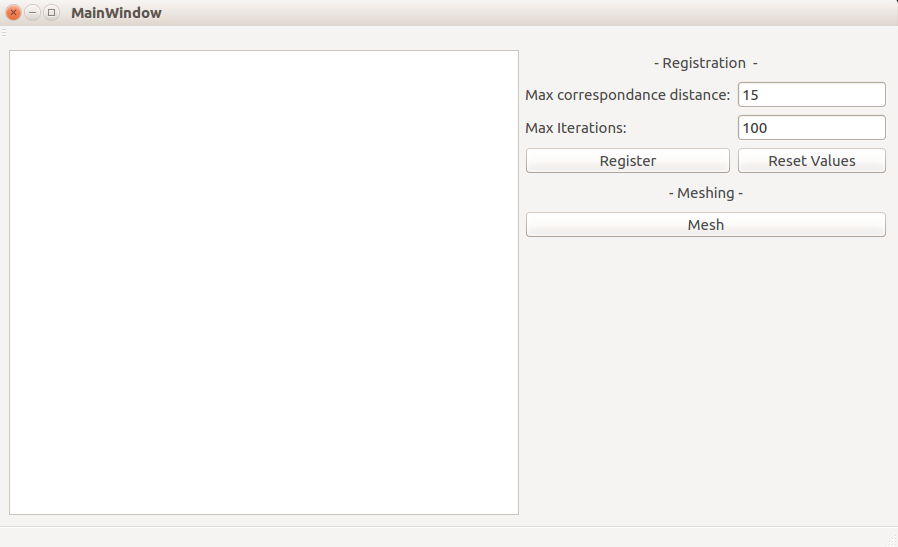
\includegraphics[width=130mm]{figures/3DCopyGUI.PNG}
	\caption{GUI:t för 3DCopy i slutet av iteration 2.}
	\label{fig:3dcopy_gui}
\end{figure}

GUI:t har 5 olika interaktioner som kan utföras. Man kan trycka på någon av de tre knapparna eller skriva i någon av de två input fälten. Det stora vita fältet är till för att visa meddelanden från mjukvaran och kan ej interageras med. Utifrån dessa 5 interaktioner kan vi ta fram EFG:n för GUI:t.

\begin{figure}[H]
	\centering
	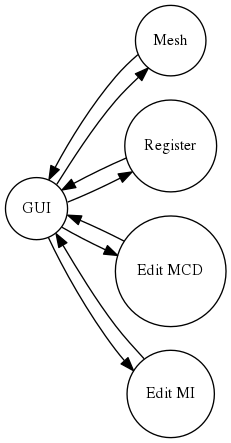
\includegraphics[width=50mm]{figures/3DCopyGUIEFG.png}
	\caption{EFG:n för 3DCopys GUI.}
	\label{fig:3dcopy_guiefg}
\end{figure}

Utifrån EFG:n ska sedan EIG:n skapas. Det som händer vid skapandet av EIG:n är att noderna GUI, Edit MCD och Edit MI tas bort eftersom att de inte interagerar med systemet.

\begin{figure}[H]
	\centering
	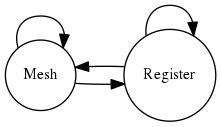
\includegraphics[width=50mm]{figures/3DCopyGUIEIG.png}
	\caption{EIG:n för 3DCopys GUI.}
	\label{fig:3dcopy_guieig}
\end{figure}

Nu när EIG:n är framtagen ska styrka väljas på testen. För att testerna ska skilja sig lite mer från de testerna utan hänsyn till kontext men åndå inte ta för lång tid väljs styrka 3 på dessa tester. Det innebär att vi får följande sekvenser som ska användas för att ta fram testfallen.

\begin{table}[h]
	\caption{De sekvenser som ska användas för att ta fram testfallen.}
	\label{tbl:test_seq}
	\centering
\begin{tabular}{|l|l|}
	\hline
	\textbf{Nr} & \textbf{Sekvens} \\
	\hline
	1 & <Mesh, Mesh, Mesh> \\
	\hline
	2 & <Mesh, Mesh, Register> \\
	\hline
	3 & <Mesh, Register, Mesh> \\
	\hline
	4 & <Mesh, Register, Register> \\
	\hline
	5 & <Register, Mesh, Mesh> \\
	\hline
	6 & <Register, Mesh, Register> \\
	\hline
	7 & <Register, Register, Mesh> \\
	\hline
	8 & <Register, Register, Register> \\
	\hline
\end{tabular}
\end{table}

Dessa sekvenser kombineras sedan för att testfallen ska uppnå 3-cover och 3\textsuperscript{+}-cover och därför också 3\textsuperscript{*}-cover. Först genererades två stycken olika  mängder med testfall som enskilt uppfyllde antingen 3-cover eller 3\textsuperscript{+}-cover. Dessa kombinerades sedan för att få fram den mängd testfall som ska utföras på GUI:t.

\begin{table}[h]
	\caption{De testfall genomfördes på GUI:t med hänsyn till kontext.}
	\label{tbl:test_context}
	\centering
	\begin{tabular}{|l|l|}
		\hline
		\textbf{Nr} & \textbf{Testfall} \\
		\hline
		1 & <Register, Mesh, Register, Mesh, Register, Mesh> \\
		\hline
		2 & <Mesh, Register, Mesh, Register, Mesh, Register> \\
		\hline
		3 & <Register, Mesh, Mesh, Mesh, Register, Mesh> \\
		\hline
		4 & <Mesh, Mesh, Register, Register, Register, Mesh> \\
		\hline
		5 & <Mesh, Mesh, Register, Mesh, Register, Mesh> \\
		\hline
		6 & <Register, Mesh, Mesh, Register, Mesh, Register> \\
		\hline
		7 & <Register, Mesh, Register, Register, Register, Mesh> \\
		\hline
		8 & <Mesh, Register, Register, Mesh, Mesh, Register> \\
		\hline
		9 & <Mesh, Register, Register, Mesh, Register, Mesh> \\
		\hline
		10 & <Mesh, Register, Mesh, Register, Register, Mesh> \\
		\hline
		11 & <Register, Mesh, Mesh, Register, Register, Mesh> \\
		\hline
		12 & <Register, Register, Mesh, Register, Mesh, Register> \\
		\hline
	\end{tabular}
\end{table}

GUI:t testas sedan genom att utföra dessa testfall i den ordning som visas i tabell \ref{tbl:test_context}. GUI:t startades om mellan varje testfall. Dessa tester utfördes manuellt på GUI:t.

\subsection{Testning av 3DCopys GUI utan hänsyn till kontext}

Som test av GUI:t utan hänsyn till kontext kan man tänka sig att en så kallad full-branch coverage kan vara tillräcklig. Det vill säga att alla olika vägar som man kan gå i GUI:t testas. Det blir alltså totalt N! antal test där N är antalet interaktioner som kan utföras på GUI:t.

\begin{table}[h]
	\caption{De testfall som genomfördes på GUI:t utan hänsyn till kontext.}
	\label{tbl:test_nocontext}
	\centering
	\begin{tabular}{|l|l|}
		\hline
		\textbf{Nr} & \textbf{Testfall} \\
		\hline
		1 & <Register, Mesh> \\
		\hline
		2 & <Mesh, Register> \\
		\hline
	\end{tabular}
\end{table}

GUI:t testas sedan genom att utföra dessa testfall i den ordning som visas i tabell \ref{tbl:test_nocontext}. GUI:t startas om mellan varje testfall. Dessa tester utfördes manuellt på GUI:t.

\section{Resultat}
\label{sec:results-holmberg}

Här presenteras de resultat som erhölls från både litteraturstudien och de tester som genomfördes på GUI:t.

Litteraturstudien visar ett tydligt samband mellan kontexten och vilka fel som testerna lyckas hitta. Kontexten är alltså avgörande för hur interaktionen kommer att påverka mjukvaran \cite{yuan2011gui}. 

\subsection{Testresultat}

I detta avsnitt presenteras de resultat som erhölls vid den testning av GUI:t som genomfördes.

\subsubsection{Med hänsyn till kontext}

Testfallen med hänsyn till kontext lyckades identifiera ett fel i meshningen. Den klarar bara av att mesha en viss fil, \textit{first\_registered\_church.pcd}. Eftersom att den tar lång tid att mesha utfördes enbart test nummer ett i tabell \ref{tbl:test_context} med denna fil. Resterande tester utfördes med andra filer som fick fel i meshningen. Alltså exekverades inte meshningskoden i de flesta fall utan bara tills felet uppstod.

\subsubsection{Utan hänsyn till kontext}

De tester som utfördes utan hänsyn till kontext hittade samma fel som de med hänsyn till kontext. Alltså att meshningen enbart klarade av en av filerna. Dessa tester utfördes båda med filer som klarade eller fick fel i meshningen.

\section{Diskussion}
\label{sec:discussion-holmberg}

I detta avsnitt diskuteras resultatet, den metod som användes samt källkritik.

\subsection{Resultat}

Som resultatet visar lyckades de båda testen identifiera samma fel trots att det med hänsyn till kontext var mycket mer omfattande. Och detta resultat kan bero på många olika saker. Dels hade systemet som testades enbart två systeminteraktioner och dessa två använder ingen delad kod. Därför är sannolikheten för att de påverkar något i koden som förstör för den andra interaktionen väldigt liten.

Dessa interaktioner är också testade sedan tidigare i andra systemtest och därför kan alla fel i koden redan vara lösta. Så sannolikheten för att det skulle finnas något fel kvar minskar ytterligare. Så det resultat som erhölls är ganska sannolikt med tanke på omständigheterna. Hade systemet varit större med fler interaktioner som delvis använder samma kod hade testningen med hänsyn till kontext eventuellt hittat fler fel.

\subsection{Metod}

En stor brist i litteraturstudien är avsaknaden av ytterligare källor. "Kontext", i kombination med testningsrelaterade termer, var de sökord som användes under sökandet av ytterligare källor. Det hade eventuellt varit fördelaktigt att utforska andra termer som beskriver kontext då inga ytterligare relevanta källor hittades. Att söka efter andra termer var dock något som inte genomfördes på grund av tidsbrist.

Den främsta bristen i metoden är att felet i meshningen inte hade hittats och blivit löst innan dessa tester. Eftersom att den enda filen som kunde meshas tog väldigt lång tid var det inte realistiskt att genomföra alla tester med den och därför är inte alla testfall med hänsyn till kontext genomförda med den filen. Det medför i sin tur att de testerna aldrig exekverade koden som utför meshningen och det kan därför finnas kontextkänsliga fel i den biten av koden som inte hittades.

Den kontextkänsliga testningen begränsades också vid t\textsuperscript{*}-cover. Det finns ytterligare ett steg som är ännu kraftfullare som kanske skulle ha hittat fel som inte identifierades.

Den kontextkänsliga testningen borde också jämförts med en annan GUI testnings metod, inte bara en testning som uppnår full path coverage. Detta för att kunna jämföra olika GUI testnings metoder.

\subsection{Källkritik}

För litteraturstudien hittades bara en relevant artikel som berörde den bit som var mest kritisk för att utföra testerna, nämligen en som tog upp hur man testar GUI:n med hänsyn till kontext. Den artikeln är skriven av personer med lång erfarenhet inom just GUI testning vilket framgick när sökandet efter ytterligare artiklar genomfördes eftersom många artiklar som dök upp var skrivna av samma personer. En anledning  till att det var svårt att hitta ytterligare artiklar kan vara att Yuan et al. \cite{yuan2011gui} har valt att kalla det för kontext. Då de också definierar begreppet kontext i sin artikel indikerar det att de eventuellt är en av få eller den enda artikeln inom just detta ämne. Eller så har andra artiklar valt en annan benämning än just kontext.

\section{Slutsatser}
\label{sec:conclusions-holmberg}

Att ta hänsyn till kontexten vid GUI testning är definitivt något som bör göras. Den är ofta avgörande för att hitta vissa fel. Det hade varit intressant att skapa exempel GUI:n med medvetet placerade fel som beror på andra interaktioner för att kunna undersöka detta noggrannare. Det fanns dock inte tid att göra en sådan undersökning i denna rapport. Därför får betydelsen av kontexter begränsas till litteraturstudien.

Gällande metoden för att ta fram testfall med hänsyn till kontext användes samma metod som i Yuan et al. \cite{yuan2011gui}. Något som blev tydligt då testerna utfördes manuellt är att metoden inte tar hänsyn till hur resurs- eller tidskrävande en interaktion är när man placerar den i sekvensen. Det är något som man skulle kunna bygga vidare på. Att undersöka hur de mest krävande interaktionerna ska placeras i sekvenserna för att testa så många kontexter som möjligt och samtidigt minimera tids- och resurskostnader.

Testerna visade att för projektets GUI, i det stadie som GUI:t befann sig i vid testningen, spelade inte kontexten någon roll för att hitta fel. Det beror sannolikt på att mängden interaktioner var liten samt att systeminteraktionerna var väl separerade och inte delade någon kod. Det indikerar att hänsyn till kontexten blir viktigare ju större mängd interaktioner GUI:t har samt hur stor del av koden som interaktionerna har gemensamt. Hade mer tid funnits skulle en undersökning med olika GUI:n med varierande antal interaktioner varit intressant för att vidare kunna undersöka denna teori.

%%%%%%%%%%%%%%%%%%%%%%%%%%%%%%%%%%%%%%%%%%%%%%%%%%%%%%%%%%%%%%%%%%%%%%
%%% holmberg-report.tex ends here

\chapter{Hur kravhanteringsmetoder påverkar ett utvecklingsprojekt}
\label{cha:indiv-report-jannering}
\chapterprecis{\LARGE{---- Gustav Jannering ----}}

\section{Inledning}
\label{sec:introduction-jannering}

Denna del redogör för projektets analysansvarige Gustav Jannerings utredning kring kravhantering och kravinsamling.

\subsection{Syfte}
\label{sec:purpose-jannering}


Syftet med denna rapport är att undersöka hur olika metoder för kravhantering och elicitering av krav påverkar ett utvecklingsprojekt av samma storlek som det projekt som övriga rapporten beskriver (ett projekt med sju till åtta utvecklare med en budget på 400 timmar vardera). Samt vilka för- och nackdelar som finns med den metoden som användes och vad som kunde gjorts annorlunda.

\subsection{Frågeställning}
\label{sec:issue-jannering}

\subsubsection{Generella frågeställningar}
\begin{enumerate}
	\item Vilka metoder finns för kravhantering och elicitering av krav och vilka fördelar och respektive nackdelar finns med dessa? 
\end{enumerate}
\subsubsection{Specifika frågeställningar}
\begin{enumerate}
	\item [2] Vilka fördelar och nackdelar finns med att använda IEEE std 830 i ett programvaruutvecklingsprojekt av den storleken som detta projekt?
	
	\item [3] Vilka erfarenheter kan dokumenteras från arbetet med krav i projektet som kan vara intressanta för framtida projekt?
	
\end{enumerate}
\subsection{Avgränsningar}
\label{sec:limits-jannering}
Denna rapport kommer att begränsas till de frågeställningar som presenterats i avsnitt \ref{sec:issue-jannering}. För metoder för elicitering av krav har följande avgränsning gjorts: endast generella metoder, metoder som går att applicera i alla situationer och som har studerats vetenskapligt ingår. Inga andra metoder (icke generella eller metoder som inte studerats vetenskapligt) kommer att presenteras i denna rapport. De erfarenheter som dokumenteras senare i denna rapport kommer uteslutande från kursen \textbf{TDDD96 	Kandidatprojekt i programvaruutveckling} och mer specifikt från det projekt i kursen som presenterats tidigare i denna rapport.   
\subsection{Definitioner, akronym och förkortningar}
\label{sec:def-jannering}
Följande definitioner och förkortningar används på flera ställen i denna del av rapporten:
\begin{itemize}
	\item Elicitering av krav - Identifiering och uppsamling av krav, översatt från det engelska ordet \textit{requirements elicitation}.
	\item Kravhantering -  arbetet med krav som ett teknisk system ska uppfylla. Översatt från det engelska ordet \textit{requirements engineering}.
	\item IEEE - Institute of Electrical and Electronics Engineers, en icke-vinstorienterad organisation bestående av ingenjörer och vetenskapspersoner. Upprätthåller standarder inom ingenjörsvetenskap.
	\item Gamification - Processen att lägga till spel eller spellika element till något (som en uppgift) för att uppmuntra deltagande \cite{lombriser2016gamified}.
	\item User story - En informell beskrivning av  funktioner i ett mjukvarusystem.
	\item Acceptance test - Ett test utfört för att avgöra om kraven i en kravspecifikation är uppfyllda.
\end{itemize}
\section{Bakgrund}
\label{sec:background-jannering}

Arbetet med kravhantering och elicitering av krav i projektet (som presenteras tidigare i denna rapport) började vid det första mötet med kunden. Detta var ett möte, dels för att träffa kunden efter att projektgruppen hade blivit tilldelade projektet, och dels för att starta kravinsamlingsfasen. Kunden i projektet, CVL, sade vid detta möte att de helst ville styra projektet med en lös hand och att det var mer eller mindre upp till projektgruppen att komma med en lista på förslag på krav (i form av ett första utkast till en kravspecifikation). För att skapa denna lista med förslag till krav på den slutgiltiga produkten så gick gruppen gemensamt igenom det projektdirektiv som CVL tidigare hade presenterat (återfinns i bilaga \ref{appendix:projekt_direktiv}), för att identifiera vilka funktioner som produkten skulle ha. Utifrån dessa funktioner kom gruppen med förslag på krav. Denna metod kallas i facklitteratur för \textit{introspektion} \cite{goguen1993techniques}. Användandet av denna metod innebar att kunden bara var involverad i att godkänna de krav som gruppen föreslog och var minimalt involverade i kravidentifieringsprocessen. 

Examinatorn i kursen (TDDD96 Kandidatprojekt i programvaruutveckling, Linköpings universitet), som detta projekt genomfördes under, hade bestämt att IEEE std 830 var den standard som kravspecifikationen skulle följa (för mer information om IEEE std 830 se kapitel \ref{sec:theory-jannering}). Detta projekt var första gången då någon i projektgruppen använde standarden, vilket medförde att vi inte hade tillräcklig kunskap för att skräddarsy standarden till projektet, istället följde vi standarden så gott vi kunde. Målet med en kravspecifikation är att identifiera kundens vision på hur den slutgiltiga produkten ska se ut och sedan tolka huruvida detta faktiskt är det som kunden vill ha eller behöver och specificera de krav som produkten ska vara bunden av. 


\section{Teori}
\label{sec:theory-jannering}
Kravhantering kan som tidigare nämnts definieras som \textit{arbetet med krav som ett teknisk system ska uppfylla}. Detta arbete ligger ofta tidigt i ett projekt, då det är viktigt att specificera de krav som skall uppfyllas. Kravhanteringsprocessen är ofta uppdelad i fyra delar: elicitering, analys, specifikation och godkännande. Detta arbete tar främst upp de tre första delarna. I detta arbete definieras elicitering som: ”insamlingen av krav eller information för senare specificering av krav från användare, kunder och andra intressenter”. I analysfasen analyseras de kraven och den informationen som samlades in under eliciteringsfasen för att undersöka huruvida dessa krav är relevanta och huruvida informationen går att använda för att specificera krav. Under specificeringsfasen ska de slutgiltiga kraven specificeras, detta innebär att varje krav numreras och att en kort text skrivs som detaljerar kravet.
\subsection{IEEE standard 830}
IEEE standard 830 är en standard, publicerad av IEEE, som specificerar innehållet och kvaliteterna hos en ”bra” kravspecifikation \cite{ieee1998ieee}. Standarden specificerar både hur en kravspecifikation borde skrivas (hur involverad kund/intressenter ska vara, hur kravspecifikationen borde utvecklas med tiden m.m.) och vilka avsnitt som borde finnas med och deras syften. Enligt IEEE ska kraven som skapas med standarden ska vara: korrekta (eller relevanta), entydiga, kompletta, konsekventa, rangordnade efter betydelse, verifierbara, modifierbara och spårbara \cite{ieee1998ieee}.

\section{Metod}
\label{sec:method-jannering}

För att undersöka vilka metoder som används för kravhantering har en litteraturstudie av publicerade vetenskapliga rapporter genomförts för att identifiera vilka metoder som har studerats och hur dessa används idag. Litteraturstudien inleddes med en litteratursökning  på universitetets biblioteksdatabas och på Googles databas, Google Scholar \cite{google_scholar}. Svårigheten med denna ansats har varit att begränsa antalet källor och försöka göra relevanta avgränsningar för att passa arbetes begränsningar. De rapporter som ingår i arbetet har uteslutande fokuserat på eliciteringsprocessen av kravhantering. Anledningen till att dessa har valts är att de uppfyller kriterierna som presenterats ovan och i avsnittet \ref{sec:limits-jannering} Vidare har endast de artiklar som presenterat eller studerat generella metoder använts. Dessa avgränsningar är gjorda för att göra denna rapport relevant för både mindre och större utvecklingsprojekt.
  
För att identifiera för- och nackdelar med IEEE std 830 \cite{ieee1998ieee} så har dels gruppen och dels analysansvariga från andra projektgrupper i denna kurs intervjuats i en öppen intervju. Se bilaga \ref{appendix:intervju_guide} för den intervjuguide som användes vid intervjuerna.

För att dokumentera erfarenheter från arbetet med kravhantering och elicitering av krav har projektgruppen gått igenom den kravspecifikation som framställdes i projektet och utvärderade vårt arbete. Erfarenheter har också dokumenterat under arbetet med denna rapport.




\section{Resultat}
\label{sec:results-jannering}
\subsection{Metoder för elicitering av krav}
På en vetenskaplig konferens i San Diego 1993 presenterade C. Linde och J. A. Goguen en rapport som beskrev författarnas undersökning och utvärdering av olika metoder för att elicitera krav \cite{goguen1993techniques}. I rapporten skriver författarna om följande metoder: Introspektion, öppna intervjuer, frågeformulär och fokusgrupper. I det följande hänvisas huvudsakligen till C. Linde och J. A. Goguen rapport \cite{goguen1993techniques}. 

\subsubsection{Introspektion}
Introspektion kallas den metod som användes i projektarbetet som presenterats tidigare i denna rapport. För att elicitera krav med introspektion så föreställer sig personen som eliciterar krav vilket system som hen skulle vilja ha om hen var kunden. Författarna skriver i sin rapport att introspektion är den mest självklara metoden för att specificera krav men att det finns fall då denna metod misslyckas med att specificera viktiga krav. Detta kan ofta bero på personliga fördomar (från eng. \textit{bias}). Två personer med olika bakgrund (både personlig och professionell) kan komma med olika krav då de använder introspektion för att elicitera krav. Det är även svårt för en enskild person att identifiera samtliga krav som bör ställas på ett system.  C. Linde och J. A. Goguens slutsats är att introspektion är en användbar metod för elicitering av krav om den kombineras med andra metoder och att de eliciterar krav med hjälp av introspektion kommer från olika bakgrunder. 

\subsubsection{Frågeformulär}
Frågeformulärsintervjuer används inom många forskningsområden. Formulär där försökspersoner får svara på frågor med förutbestämda svar är ett bra sätt för forskare att få statistisk information. Detta tillvägagångssätt kan anpassas för att användas för att elicitera och specificera krav. Tänkta användare, kunder och andra intressenter får, med hjälp av den som eliciterar krav, fylla i ett formulär, vars data senare analyseras för att identifiera vad som är relevant för de som svarade på formuläret. Liksom i forskningsvärlden så är detta ett sätt att få statistisk information som kan visas för kunden och användas som underlag i en mängd situationer under utvecklingen av ett system. Författarna poängterar att det finns ett fundamentalt problem med detta tillvägagångssätt, -Vad händer om den som skapar formuläret och frågorna, och den som svarar på frågorna inte har samma referensram?.
 
\subsubsection{Öppna intervjuer} 
 C. Linde och J. A. Goguen kommer fram till att ett sätt att lindra problemet med frågeformulärsmetoden är att istället hålla s.k. öppna intervjuer. Intervjuaren ställer en fråga och låter försökspersonen svara på frågan med egna ord. Intervjun fortskrider med ett antal förutbestämda frågor som ska ställas och besvaras men intervjuaren kan ställa följdfrågor och egna frågor emellan de förskriva frågorna. Denna metod används ofta av psykologer och andra som forskar inom liknande områden. För att anpassa denna metod för elicitering av krav ändrar man vilka frågor man ställer och vilka personer man ställer frågorna till. Frågorna kommer att handla om hur försökspersonen använder system som liknar det system som ska utvecklas. Det är viktigt att frågorna är konstruerade så att de inte leder till att försökspersonen använder introspektion för att själv föreställa vilka krav som personen tycker systemet bör ha. Försökspersonerna kommer, liksom med frågeformulärsmetoden, att vara tänkta användare, kunder och andra intressenter. 

\subsubsection{Fokusgrupper}
Den sista metoden för elicitering av krav som C. Linde och J. A. Goguen presenterar i sin rapport är fokusgrupper (från eng. \textit{focus groups}). Fokusgrupper är mycket vanligt i marknadsundersökningar. Tanken bakom fokusgrupper är att samla en grupp intressenter (potentiella kunder om en marknadsundersökning utförs) med olika bakgrunder. Gruppen får sen diskutera ett ämne som är av intresse (t.ex. en ny produkt om en marknadsundersökning utförs). Arrangören för protokoll på vad som sägs i gruppen och använder senare denna data som underlag vid beslut \cite{hylander1998fokusgrupper}. För att applicera denna metod för att elicitera krav så skapas JAD- (\textit{Joint Application Development}) eller RAD- (\textit{Rapid Application Development}) grupper bestående av utvecklare, kunder och andra intressenter som i grupp diskuterar det system som ska utvecklas. Författarna poängterar att det är svårt att inkludera personer som saknar teknisk bakgrund i dessa samtal då de har svårigheter att bedöma betydelsen av tekniska beslut. Författarnas slutsats är att denna metod är lovande men att dess begränsningar bör studeras. 

\subsubsection{GREM}
I en rapport som presenterades på International Working Conference on Requirements Engineering: Foundation for Software Quality i Göteborg 2016 skriver P. Lombriser et al. \cite{lombriser2016gamified} om en ny metod för elicitering av krav som bygger på gamification. Rapporten beskriver metod som ska öka engagemanget hos interessenter vid elicitering av krav som författarna kallar \textit{gamified requirements engineering model} eller \textit{GREM}. I rapporten presenterar författarna ett experiment där en webbaserad plattform, som har spellika element, använts för att elicitera krav genom att skapa user stories och acceptence tests. Författarnas slutsats är att deras experiment visar att användandet av spellika element kan ha en positiv inverkan på intressenters engagemang men att denna inverkan kan variera baserat på vilka spellika element som används.

\subsubsection{Kravkategorisering}
I sin doktorsavhandling definierar M. Karlsson tre olika kategorier för krav: \textit{fångade krav} (från eng. captured requirements), \textit{eliciterade krav} (från eng. elicited requirements) och \textit{framväxande krav} (från eng. emergent requirements)\cite{lkp.26083619960101}. \textit{Fångade krav} är krav som är relativt lätta att specificera eller som är relativt uppenbara. \textit{Eliciterade krav} är krav som identifierats efter att grävt djupare i vad som tänkta användare, kunder och andra intressenter förväntar sig av systemet. Dessa krav kan klassas som icke uppenbara och kräver en grad av utredning för att identifieras. \textit{Framväxande krav} är krav som växer fram under utvecklingen av systemet allt efter att tänkta användare, kunder och andra intressenter fått testa systemet. Dessa krav är svåra att identifiera i ett utvecklingsprojekts tidiga stadier om utvecklingsgruppen inte håller prototypdemonstationer där tänkta användare får komma med feedback. 
 
\subsection{Erfarenheter}
\label{sec:expreience-jannering}
Följande är en sammanfattning av de erfarenheter om kravhantering och elicitering av krav som dokumenterats under projektets gång.
\begin{itemize}
	\item Att skapa en \textit{bra} kravspecifikation är svårt.
	\item För att identifiera relevanta krav gäller det att både utvecklingsgruppen och kunden är tillräckligt insatta i det som ska utvecklas. (speciellt om projektets mål är att vidareutveckla ett system).
	\item Att blint följa IEEE std 830 för att skriva en kravspecifikation kan vara frustrerande.
	\item Kunden (och/eller tänkta användare) borde vara mer involverad vid specificering av krav än de var i projektet.
	\item Vid vidareutveckling är det viktigt att testa det befintliga systemet ordentligt innan man specificerar krav.
\end{itemize}

\subsection{IEEE standard 830}
Följande är en sammanfattning av två öppna intervjuer gjorda med två analysansvariga från två olika grupper i kursen \textbf{TDDD96 	Kandidatprojekt i programvaruutveckling}. Intervjuguiden som användes vid dessa intervjuer återfinns i bilaga \ref{appendix:intervju_guide}. Svaren på intervjuerna är anonymiserade.  

Båda intervjuobjekten använde introspektion för att elicitera krav i sina projekt. De började med att analysera det projektdirektiv som gavs för respektive projekt, eliciterade krav utifrån dessa och skapade ett första utkast till en kravspecifikation som de sedan skickade till sina respektive kunder. När det gäller användandet av IEEE std 830 svarade det ena intervjuobjektet att de inte använt sig av denna standard vid skrivandet av kravspecifikationen. Intervjuobjektets grupp baserade sin kravspecifikation på en mall från en tidigare projektkurs och undersökte IEEE std 830 först efter att en opponerande grupp hade påpekat att IEEE std 830 var standarden som skulle användas. Det andra intervjuobjektets grupp använde sig av IEEE std 830 från början. Efter utfrågning om vad de tyckte om standarden höll båda intervjuobjekten med om att standarden gav en bra mall att följa när det gällde vilka rubriker som bör vara med i en kravspecifikation men att standarden kändes för omständlig för ett projekt av denna omfattning och att de kände att det tog för lång tid att läsa igenom och sätta sig in i standarden.          

\section{Diskussion}
\label{sec:discussion-jannering}

\subsection{För- och nackdelar med metoder för elicitering av krav}
Nedan används M. Karlssons kravkategorisering för att diskutera vilka metoder som är kapabla att specificera vilka krav. Den tredje kategorin av krav, \textit{framväxande krav}, är mycket svåra att korrekt identifiera tidigt i ett projekt så den kommer inte att användas.
\subsubsection{Introspektion}
Min åsikt om för- och nackdelarna med introspektion stämmer överens med C. Lindes och J. A. Goguens slutsats om introspektion \cite{goguen1993techniques}. Introspektion är en bra metod för elicitering av krav om den kombineras med andra metoder och att de som eliciterar krav med hjälp av introspektion kommer från olika bakgrunder. Ren introspektion kräver mycket erfarenhet för att kunna elicitera alla relevanta krav som bör ställas på ett system. Introspektion klarar i nästan alla fall att identifiera alla \textit{fångade krav}, eftersom de kraven är mer eller mindre uppenbara. Men det krävs en betydande mängd erfarenhet för att identifiera samtliga \textit{eliciterade krav}.

\subsubsection{Frågeformulär}
Frågeformulär, liksom introspektion, är beroende av att den som eliciterar krav (och i detta fall skapar frågorna och svaren) har en korrekt bild av vad kunden, tänkta användare och andra intressenter vill ha för system. Om denna bild inte är korrekt finns det en stor risk att de krav som eliciteras inte är relevanta. Liksom introspektion klarar frågeformulär av att elicitera \textit{fångade krav}, men om den som skapar frågorna och svaren, och försökspersonen inte delar samma referensram så finns risken att vissa \textit{eliciterade krav} missas. 

\subsubsection{Öppna intervjuer}
Användandet av öppna intervjuer lindrar problemet med frågeformulärsmetoden. Om intervjuaren och försökspersonen inte har samma uppfattning om vad som ska utvecklas eller vilka systemets fundamentala aspekter är så finns risken att kraven som specificeras med hjälp av intervjun inte är relevanta. Öppna intervjuer kommer nästan alltid att identifiera alla \textit{fångade krav}, men liksom frågeformulär finns det en risk att vissa \textit{eliciterade krav} inte specificeras. Ett annat problem med denna metod är tidsaspekten. Öppna intervjuer tar tid. Eftersom intervjuerna görs en och en kommer tiden det tar att elicitera krav från samma mängd intressenter att ta mycket längre tid om man använder öppna intervjuer istället för frågeformulär.  

\subsubsection{Fokusgrupper}
En risk med fokusgrupper är att deltagarna i gruppen inte representerar verkligheten, d.v.s. att deltagarna inte lyckas representera en eller flera grupper av intressenter, vilket leder till att vissa relevanta krav inte identifieras. Det finns också andra risker med fokusgrupper. Eftersom en fokusgrupp ska starta en diskussion kring ett ämne så finns risken att en minoritet av gruppen inte blir hörda eller att delar av gruppen hörs för mycket. Det kan vara lätt för en majoritet att utesluta en minoritet från diskussionen eller att en minoritet tar över diskussionen. Detta kan leda till att de som representerar en grupp intressenter inte blir hörda och att relevanta krav inte blir eliciterade. Fokusgrupper har enligt min uppfattning störst chans att korrekt identifiera samtliga \textit{eliciterade krav} så länge gruppen fungerar korrekt.

\subsubsection{GREM}
GREM verkar vara en lovande metod men den är väldigt ung (rapporten som presenterade metoden skrevs 2016) och är beroende av extern mjukvara. GREM har potential men bör studeras mer och/eller standardiseras innan den används mer brett. I teorin har GREM potentialen att korrekt identifiera alla \textit{eliciterade krav} i form av user stories och acceptance tests skapade av kunder, eftersom GREMs mål är att involvera kunder, användare och andra intressenter i eliciteringsprocessen.

\subsection{För- och nackdelar med IEEE std 830}
Att intervjua två personer för att identifiera för- och nackdelar med en standard som är skapad av en organisation med tusentals medlemmar, och som har mycket större kunskap och erfarenhet av ämnet, är inte optimalt, men det kan ge en bra bild av hur personer som försöker sätta sig in i standarden känner. Efter intervjuerna och efter att ha reflekterat över mina egna erfarenheter av standarden kan jag konstatera att våra åsikter om standarden är väldigt lika. IEEE std 830 ger en bas att bygga en välkonstruerad kravspecifikation på men i detta fall, ett mindre projekt med relativt få projektmedlemmar, känns standarden överflödig.   
\subsection{Erfarenheter}
Erfarenheterna som finns listade i avsnitt \ref{sec:expreience-jannering} är specifika för detta projekt, ett projekt där kraven fick skrivas om efter det att fel med den befintliga mjukvaran som skulle vidareutvecklas hittats. Detta är ett tveeggat svärd, dels ger det bra erfarenheter att se tillbaka på om hur vi borde ha gjort för att identifiera dessa fel tidigare. Men det som ledde till att vi inte identifierade felet i ett tidigt skede var en serie av val (både från vår och från kundens sida) som där och då verkade försumbara, men som i efterhand visar att vi, från gruppens sida, borde ha ställt högre krav på kundens kunskap om systemet innan vi specificerade krav på vår vidareutveckling av den befintliga mjukvaran som implicit antog att den befintliga mjukvaran var relativt felfri. Med detta i åtanke skulle jag hävda att de erfarenheter som är listande i avsnitt \ref{sec:expreience-jannering} alla är relevanta erfarenheter för framtida projekt.      
\subsection{Källkritik}
De källor som använts i denna rapport är alla publicerade källor som citerats i tidigare arbeten. Den första källan som har använts är publicerad av IEEE, som nämns i avsnitt \ref{sec:def-jannering} är IEEE en icke-vinstdrivande organisation som upprätthåller standarder inom ingenjörsvetenskap. Den andra källan är publicerad av ett stort förlag och presenterades dessutom på en internationell konferens. Den tredje och sista är en doktorsavhandling från Chalmers. Ovanstående leder mig till att anse att dessa källor är pålitliga.      
\subsection{Alternativa metoder}
Det finns en uppsjö  med metoder som skulle kunna ha använts för att besvara de frågor som ställs i avsnitt \ref{sec:issue-jannering} inom ramen för detta arbetes begränsningar. Problemet i detta fall har varit att finna metoder för att besvara frågorna som passade detta arbetets tidsbegränsningar. Av denna anledning valdes just en begränsad litteraturstudie tillsammans med öppna intervjuer och en utvärdering för att besvara frågorna. Om tidsbegränsningen för detta arbete varit annorlunda kunde man utvidgat både litteraturstudien och de öppna intervjuerna.   
\section{Slutsatser}
I det följande kommer slutsatserna att redovisas i samma följd som frågorna i avsnitt \ref{sec:issue-jannering}
\label{sec:conclusions-jannering}
\subsection{Vilka metoder finns för kravhantering och elicitering av krav och vilka fördelar och nackdelar finns med dessa?}
De metoder för elicitering av krav som presenterats är: introspektion, frågeformulär, öppna intervjuer, fokusgrupper och GREM.

\subsubsection{Introspektion}
Introspektion är den vanligaste metoden för att elicitera krav men min slutsats är att i många fall är detta inte den bästa metoden att använda. Det finns för många felkällor med denna metod för att säga att man borde använda ren introspektion (bara introspektion) för att elicitera krav. Metoden bygger på att den som eliciterar krav lyckas få en komplett bild av det system som kunden/användaren vill ha. Denna bild kommer att vara komplex, även i mindre projekt, vilket betyder att många eliciterade krav kan falla bort på vägen.

\subsubsection{Frågeformulär}
Frågeformulär har fördelen att kunna samla in statistisk information om vad kunder/användare vill ha för system men som tidigare presenterats finns ett ganska fundamentalt problem med denna metod: Vad händer om den som skapar formuläret och frågorna och den som svarar på frågorna inte har samma referensram?. Min slutsats är att frågeformulär är en bättre metod för att elicitera krav än introspektion då man involverar kunder och användare mer, men att även den är bristfällig.

\subsubsection{Öppna intervjuer}
Öppna intervjuer kan vara en bättre metod för elicitering av krav eftersom kunder och användare är mer engagerade i eliciteringsprocessen. Dock finns det två problem med metoden. Dels samma problem som med frågeformulär (och introspektion) och dels tidsaspekten. Att utföra tillräckligt många öppna intervjuer för att identifiera alla relevanta krav kan ta för lång tid och kosta för mycket för ett mindre utvecklingsprojekt.

\subsubsection{Fokusgrupper}
Fokusgrupper har potentialen att vara den bästa metoden för elicitering av krav (så länge en eller flera gruppen, med rätt komposition, kan samlas). Fokusgrupper lider inte av samma problem med tid som öppna intervjuer och den referensram som gruppen har borde vara uppenbar efter att gruppen har träffats. Problemen med fokusgrupper (som presenterats tidigare) och C. Lindes och J. A. Goguens slutsats, att metodens begränsningar bör studeras, får mig att tveka att rekommendera metoden \cite{goguen1993techniques}.

\subsubsection{GREM}
GREM är den metod som är svårast för mig att rekommendera. Utifrån den data som presenterats av P. Lombriser et al. \cite{lombriser2016gamified} verkar metoden lovande men eftersom metoden är beroende av extern mjukvara för elicitera krav och metoden är så pass ny så kan jag inte komma till slutsatsen att denna metod kan rekommenderas.

\subsubsection{Sammanfattning}
Alla metoder har sina egna styrkor och svagheter.

Det bästa tillvägagångssättet för att elicitera krav är att använda flera av de metoder som presenterats för att säkerställa att alla krav som bör ställas på ett system identifieras och specificeras.        

\subsection{Vilka fördelar och nackdelar finns med att använda IEEE std 830 i ett programvaruutvecklings projekt av den storleken som detta projekt?}
IEEE std 830 ger en bra översikt över vad som bör vara med i en välkonstruerad kravspecifikation, men att dessa fördelar inte väger upp hur lång tid det tar att sätta sig in i standarden för utvecklare i ett mindre projekt. Efter att ha läst igenom standarden förstår man hur väluttänkt den är. Problemet med standarden är att det tar lång tid att sätta sig in i. Tid som kan vara knapp i början av ett projekt. 
\subsection{Vilka erfarenheter kan dokumenteras från kravhantering och elicitering av krav i projektet som kan vara intressanta för framtida projekt?}
De erfarenheter som har kunnat dokumenteras kring ämnet kravhantering och elicierting av krav är följande:
\begin{itemize}
	\item Att skapa en välkonstruerad kravspecifikation är svårt.
	\item För att identifiera relevanta krav gäller det att både utvecklingsgruppen och kunden är tillräckligt insatta i det som ska utvecklas (speciellt om projektets mål är att vidareutveckla ett system).
	\item Att blint följa IEEE std 830 för att skriva en kravspecifikation kan vara frustrerande.
	\item Kunden (och/eller tänkta användare) borde vara mer involverad/de vid specificering av krav än de var i projektet.
	\item Vid vidareutveckling är det viktigt att testa det befintliga systemet ordentligt innan man specificerar krav.
\end{itemize}


%%%%%%%%%%%%%%%%%%%%%%%%%%%%%%%%%%%%%%%%%%%%%%%%%%%%%%%%%%%%%%%%%%%%%%
%%% Jannering-report.tex ends here

\chapter{Analys av punktmolnsregistrering}
\label{cha:indiv-report-karlsson}
\chapterprecis{\LARGE{---- Michael Karlsson ----}}


\section{Inledning}
\label{sec:introduction-karlsson}

%% Skriv här
I detta kapitel behandlas Michael Karlssons undersökning av olika registreringsalgoritmer och de problem gruppen stött på i samband med registrering av punktmoln.

\subsection{Syfte}
\label{sec:purpose-karlsson}

%% Skriv här
Syftet med denna delen är att väga olika algoritmer mot varandra och hur väl de fungerade för det projekt som beskrivs i rapporten samt vilka problem gruppen hade med de olika algoritmer som testades. Gruppens tillvägagångssätt för val av algoritm undersöks också.


\subsection{Frågeställning}
\label{sec:issue-karlsson}

\begin{itemize}
	\item Hur skapar man ett enhetligt punktmoln från enstaka bilder från en fast \newline avståndskamera?
	\item Hur gör man för att välja algoritm och hur resonerade gruppen när de valde ICP?	
\end{itemize}

\subsection{Definitioner och förkortningar}
\label{sec:definitions-acronyms-karlsson}

Här listas de definitioner och förkortningar som används i kapitlet.

\begin{itemize}
	\item Point Cloud Library - Ett C++ bibliotek för hantering av punktmoln.
	\item PCL - Point Cloud Library.
	\item Iterative Closest Point - En algoritm för punktmolnsregistrering.
	\item ICP - Iterative Closest Point.
	\item JR-MPC - Joint Registration of Multiple Point Clouds
	\item SeqICP - SequentialICP
\end{itemize}


\subsection{Avgränsningar}
\label{sec:limits-karlsson}
Denna rapport kommer begränsas till hur processen fungerat med den hårdvara som vi blivit tilldelade. För registrering finns en ofantlig mängd algoritmer och tillvägagångssätt. Denna utredning kommer begränsas till de metoder som använts inom projektet. 


\section{Bakgrund}
\label{sec:background-karlsson}
I ett tidigt stadie av projektet upptäckte vi att en stor del skulle handla om att få registreringen att funka bra. Tidiga tester visade dessutom att meshningen, en annan del som tidigt verkade väldigt stor, som görs efter registreringen var förhållandevis enkel att utföra. Meshning innebär att man, utifrån det kompletta punktmolnet, skapar en vattentät 3D-modell. Jag blev intresserad efter att ha jobbat en del med tidiga försök till registrering och beslutade mig för att djupdyka i ämnet.


\section{Teori}
\label{sec:theory-karlsson}

När man vill återskapa fysiska objekt digitalt fastnar man oftast i att det inte finns några bra verktyg för att läsa in tredimensionella objekt. Man behöver då ta flera bilder av objektet från olika vinklar för att kunna sammanfoga dessa till det fulla objektet. Det finns många metoder för detta, exempelvis Kinect Fusion. Den metod vi använt oss av har dock bestått av en avståndskamera på linjärenhet med objektet monterat på ett rotationsbord med 2 rotationsaxlar. Med hjälp av detta rotationsbord kan men förhållandevis enkelt se hela objektet från en fast punkt. Dessa punktmoln har vi haft som moln att enhetligt registrera till en komplett representation av objektet som skannats.


\subsection{Registrering}

Registrering är den generella metoden att sätta ihop två eller flera punktmoln till ett koordinatsystem med all information från indatan. Det finns väldigt många olika algoritmer för att utföra detta såsom till exempel ICP, \textit{Iterative Closest Point} eller GMMReg. De flesta tillgängliga algoritmer har någon form av svaghet eller nackdel. Till exempel så lider ICP av så kallad \textit{felutbredning} och JR-MPC \textit{Joint Registration of Multiple Point Clouds} lider av längre körtid.[]

\subsection{Kinect Fusion}

Kinect fusion använder sig av Microsofts egna avstånds- och RGB-kamera, Kinect, för att mappa upp ett 3D objekt i den verkliga världen. Avståndskameran mäter upp punktmolnet för scenen framför den samtidigt som den synkroniserade RGB-kameran ger färgdata till varje punkt. 
Varje punktmoln som Kinect kameran skickar består av ca 307 000 punkter. Det kan jämföras med hårdvaran som vi använt oss av där maximala antalet punkter i en skanning är ca 786 000 punkter. De punktmoln som vi arbetat med har dock generellt innehållit ca 30-60 000 punkter efter filtrering av skräpdata.

\section{Metod}
\label{sec:method-karlsson}

Initialt gjordes en litteraturstudie för att hitta information om hur man registrerar. PCL ger en bra sammanfattning men utöver det finns inte jättemånga relevanta källor. PCL ger också många handledningsexempel med exempelkod som blev utgångspunkten för utbildningen om registrering i gruppen. Då utredningen är begränsad till framförallt ICP och JR-MPC begränsas antalet ytterligare. Det finns enormt många varianter av ICP, såsom SeqICP, Point-to-Plane ICP Point-to-Point ICP m.fl. Jag har inte hittat någon referens i PCL, vars ICP-implementation gruppen använder sig av, till vilken av dessa PCL implementerar. På grund av det här kommer en generell ICP algoritmen utvärderas. JR-MPC är resultatet av en forskningsstudie som tagit fram algoritmen och därmed finns enbart den källa som används här för den algoritmen. Det finns snarlika algoritmer med enbart sina forskningsdokument som källa men dessa kommer alltså inte behandlas här.



\section{Resultat}
\label{sec:results-karlsson}

%% Skriv här
Vi började med att införskaffa oss en uppsättning punktmoln på objektet och försökte med den exempelkod vi hittat sätta ihop punktmolnen. De första objektet vi började testa med var en porslinskyrka pga att det var det enda vi hade att tillgå. Efter ett par veckor fick vi en låda med träklossar som vi började arbeta med och som blev vårat primära mål att registrera då dessa rekommenderades av kund som lättare objekt.
 Den primära algoritm vi använde var ICP. Valet av ICP var initialt baserat på att det var den algoritm vi hittade först samt den som vi fick tag på exempelkod för. Vi gjorde dock vissa begränsade tester med JR-MPC som rekommenderades av kunden CVL. Då JR-MPC inte vid tidpunkten gav bättre resultat än den metod som användes samt betydligt mer manuellt arbete för att kunna köra algoritmen så lades snabbt arbetet med JR-MPC på is. Mer fokus lades på att jobba vidare med ICP och ungefär halvvägs in i projektet hade vi en algoritm som funkade på ca 20 av de 36 punktmoln på objektet. Efter det hamnade ett 

\subsection{ICP}
ICP är en optimeringsalgoritm som försöker minimera det totala avståndet från varje punkt i ursprungsmolnet till varje punkt i målmolnet. Det ger en bästa körtid på $ \mathit{O(n^2)} $
\subsection{JR-MPC}
JR-MPC använder så kallade GMM, \textit{Gaussian Mixture Model}, för att registrera objektet. Exakt hur matematiken bakom algoritmen ser ut och fungerar är utanför omfattningen av denna rapport. Genom att ta fram sannolikheten för att en punkt ligger inom objektet som ska 

\subsection{3DCopy metoden}
Under utvecklingsarbetet och problemfaser med registreringen planerade gruppen om och försökte med en annan lösningsmetod till registreringsproblemet. Då registreringsalgoritmerna som använts helt ignorerar den kända datan om hur mycket rotation som skett mellan varje skanning så blev det fokus för våran metod. 

\section{Diskussion}
\label{sec:discussion-karlsson}

\subsection{Diskussion om Metod}

\subsection{Diskussion om Resultat}

\subsection{Diskussion om Metod}


\section{Slutsatser}
\label{sec:conclusions-karlsson}

%% Skriv här

%%%%%%%%%%%%%%%%%%%%%%%%%%%%%%%%%%%%%%%%%%%%%%%%%%%%%%%%%%%%%%%%%%%%%%
%%% karlsson-report.tex ends here

\chapter{Att bygga ett system i ROS av Martin Lundberg}
\label{cha:indiv-report-person}

\section{Inledning}
\label{sec:introduction-person}



\subsection{Syfte}
\label{sec:purpose-person}

%% Skriv här

\subsection{Frågeställning}
\label{sec:issue-person}

Hur kan en arkitektur implementeras i ROS?

Hur hade arkitekturen för systemet sett ut utan ROS?

\section{Bakgrund}
\label{sec:background-person}

%% Skriv här

\section{Teori}
\label{sec:theory-person}

%% Skriv här

\section{Metod}
\label{sec:method-person}

%% Skriv här

\section{Resultat}
\label{sec:results-person}

%% Skriv här

\section{Diskussion}
\label{sec:discussion-person}

%% Skriv här

\section{Slutsatser}
\label{sec:conclusions-person}

%% Skriv här

%%%%%%%%%%%%%%%%%%%%%%%%%%%%%%%%%%%%%%%%%%%%%%%%%%%%%%%%%%%%%%%%%%%%%%
%%% person-report.tex ends here

\chapter{Verktyg som är lämpliga för att skriva stora dokument}
\label{cha:indiv-report-tuhkala}
\chapterprecis{\LARGE{---- Hannes Tuhkala ----}}

\section{Inledning}
\label{sec:introduction-tuhkala}
Att skapa bra och stiliga dokument är viktigt för att det ska se professionellt ut. I den här rapporten kommer en undersökning som är gjord av Hannes Tuhkala om vilka fördelar och nackdelar som \latex och Word har för att skriva stora dokument. Rapporten tar också upp vilka verktyg som lämpar sig för att skriva stora dokument.

\subsection{Syfte}
\label{sec:purpose-tuhkala}
Syftet med den här rapporten är att ta reda på vilka för- respektive nackdelar som finns med att använda \latex och Word för att framställa dokument. Syftet är också att undersöka vilka asynkrona eller synkrona verktyg som är lämpliga att använda för att skriva stora dokument samt vilka erfarenheter projektgruppen kan ta med sig ifrån projektet gällande dokumenthantering.

\subsection{Frågeställning}
\label{sec:issue-tuhkala}
De frågeställningar som rapporten behandlar är:

\begin{enumerate}
	\item Vilka fördelar och nackdelar finns det med att använda \latex eller Word när man skriver dokument?
	\item Vilka verktyg lämpar sig för att skriva större dokument?
	\item Vilka erfarenheter kan tas med ifrån det här projektet gällande framställning av större dokument?
\end{enumerate}

\subsection{Definitioner, akronym och förkortningar}
Följande definitioner och förkortningar används på flertalet ställen i den här rapporten:

\begin{itemize}
	\item Ett större dokument - Definierar här som ett dokument som två eller flera personer arbetar på och är åtminstone sju sidor långt.
	\item Synkront verktyg - Ett program eller en tjänst som flera personer kan skriva samtidigt på utan att man behöver vänta på att någon annan skrivit färdigt.
	\item Asynkront verktyg - Ett program eller en tjänst som en person skriver text på och skickar det till andra personer efteråt.
	\item SVN - Apache Subversion
	\item Word - Microsoft Word
	\item WYSIWYG-editor - WYSIWYG står för (What You See Is What You Get) och en sådan editor är ett program eller system där innehåll kan ändras på ett sådant sätt att det liknar hur det slutgiltiga dokumentet kommer att se ut.
	\item Separata filer - Se avsnitt \ref{sec:thesis-info-tuhkala}.
	\item Gemensam fil - Se avsnitt \ref{sec:thesis-info-tuhkala}.
	\item Linter - En linter är ett verktyg som flaggar misstänkta fel i kod med avseende på vad som är tillåtet i programmeringsspråket \cite{linter}.
\end{itemize}

\subsection{Avgränsningar}
Denna rapport kommer endast att ta upp de två vanligaste typsättningssystemen, \latex och Microsoft Word eftersom de är de mest använda och kända. Det finns liknande system som dessa, till exempel OpenOffice eller LibreOffice och de kommer inte att behandlas i rapporten för att de inte är lika välanvända och kända. Rapporten kommer också att ta upp olika asynkrona verktyg som Git, SVN och Mercurial samt synkrona verktyg som Google Docs, ShareLaTeX och Overleaf. Dessa valdes också för att de är de vanligaste tjänsterna och mest använda.

\section{Bakgrund}
\label{sec:background-tuhkala}
Vi har arbetat med olika verktyg för att framställa större dokument för projektet i gruppen. Vi har använt oss av \latex för alla våra större dokument och använt oss av både asynkrona och synkrona verktyg när vi skrev dessa. För alla större dokument utom kandidatrapporten användes ett synkront verktyg, Overleaf. För kandidatrapporten använde vi oss av ett asynkront verktyg, Git. Den här studien har genomförts för att se vilket av de olika asynkrona och synkrona verktygen som kan vara bättre att använda sig utav för större dokument. Flera andra verktyg har också tagits upp för att se hur andra projektgrupper framställer sina dokument. 

\section{Teori}
\label{sec:theory-tuhkala}
Nedan visas information om det som kommer att tas upp i rapporten. Det ger lite teori om vad \latex, Git och SVN är för något.

\subsection{\latex}
\latex är ett typsättningssystem som är baserat på TeX och skapades för att göra det enklare att skapa generella böcker och artiklar inom TeX. Till skillnad från till exempel Microsoft Word, programmerar man dokumentet, istället för att skriva formaterad text. \latex bygger på att den som skriver inte ska formatera texten, utan ska bara skriva det den vill få sagd, utan att behöva bry sig om hur dokumentet ser ut. Det är därför väldigt enkelt att få stiliga dokument i \latex genom att bara specifiera dokumentets struktur istället för att krångla med hur dokumentet ska se ut.

\subsection{Git}
Git \cite{git}\cite{git_history} är ett versionshanteringsprogram som skapades av Linus Torvalds för att hantera källkoden till Linuxkärnan. Git är ett så kallat distribuerat versionshanteringssystem, vilket innebär att alla som använder ett Git repository har allt som det innehåller och behöver inte använda en centraliserad server. Git har också komplett historik över alla ändringar som skett och man kan gå tillbaka till tidigare versioner av dokument och källkod.

\subsection{Apache Subversion}
Subversion (SVN) \cite{svn} är också ett versionshanteringsprogram för mjukvara likt Git, förutom att SVN är ett centraliserat versionshanteringssystem.

\subsection{Mercurial}


\subsection{Kandidatrapport}
\label{sec:thesis-info-tuhkala}
Kandidatrapporten är skriven i \latex och använder mallen för avhandlingar skapad av Ola Leifler \cite{thesis_template}. Mallen är upplagd så att det finns separata filer för varje del av rapporten istället för en enstaka stor fil. Det innebär att introduktion, bakgrund, metod, de individuella bidragen samt de andra delarna i rapporten är separata filer.

\section{Metod}
\label{sec:method-tuhkala}
För att kunna besvara frågeställningarna har jag delat upp dem i tre sektioner för hur jag gick tillväga för att svara på dem.

\subsection{Första frågeställningen}
För min första frågeställning gjordes en litteraturstudie för att samla information om vilka för- och nackdelar som finns med att använda \latex eller Word när man skriver dokument. Detta för att se hur tidigare arbeten ställer sig till sde två olika typsättningssystemen som jag tar upp i frågeställningen.

\subsection{Andra frågeställningen}
För min andra frågeställning gjordes en enkätundersökning som skickades ut till alla som läser kursen TDDD96, Kandidatprojekt i programvaruutveckling. I enkäten ställdes först dessa frågor:
\begin{itemize}
	\item Vilken grupp är du i?
	\item Vilket verktyg använder ni när ni skriver de flesta större/viktiga dokument?
\end{itemize}
Beroende på hur de svarade på föregående fråga "Vilket verktyg använder ni när ni skriver de flesta större/viktiga dokument?" får de olika frågor. Om de valde alternativ 1 (Asynkrona verktyg som Git, SVN och liknande) fick de följande frågor:
\begin{itemize}
	\item Vad för slags versionshanterare använder ni er av?
	\item Hur nöjd är du med hur ni versionshanterar era dokument?
	\item Om du fick ändra vilket asynkront versionshanteringsverktyg ni använde, vilket hade du då valt?
	\item Skulle du vilja byta hantering av dokument till synkrona verktyg som Google Docs, ShareLaTeX och liknande?
	\item Om du svarade ja, vilket verktyg skulle du då vilja använda?
\end{itemize}
Om de valde alternativ 2 (Synkrona verktyg som Google Docs, ShareLaTeX och liknande) fick de besvara dessa frågor istället:
\begin{itemize}
	\item Vilken webbsida/tjänst använder ni er av för större/viktiga dokument?
	\item Hur nöjd är du med att använda en tjänst som denna för hantering av dokument?
	\item Om du fick byta den tjänst ni använde, vilken hade du då valt?
	\item Skulle du vilja byta hantering av dokument till asynkrona verktyg som Git och SVN?
	\item Om du svarade ja, vilket verktyg skulle du då vilja använda?
\end{itemize}
Till sist frågades också detta oberoende av vilka alternativ man valt.
\begin{itemize}
	\item Vilka verktyg som har listats här tycker du är bra för större dokument?
\end{itemize}

\subsection{Tredje frågeställningen}

För min tredje frågeställning gjordes också en enkätundersökning men enbart för medlemmarna i projektgruppen. Där ställdes dessa frågor:
\begin{itemize}
	\item Överlag hur tycker du att hanteringen av större dokument har gått i gruppen?
	\item Vilket verktyg tycker du har varit bäst att använda?
	\item Varför tycker du det?
	\item För kandidatrapporten, tycker du att det var bättre med separata filer än en gemensam fil?
\end{itemize}

\section{Resultat}
\label{sec:results-tuhkala}
Resultatet som jag kommit fram till från min litteraturstudie och de två enkäter som beskrevs i metoden visas nedan.

\subsection{Litteraturstudie}
Knauff och Nejasmic \cite{knauff2014efficiency} visar med hjälp av ett mjukvaruanvändbarhetstest hur effektivt det är att använda sig av \latex jämfört med Microsoft Word. Testet gick ut på att 40 deltagare över olika vetenskapsgrenar skulle skriva olika vetenskapliga texter.
Det visar sig att \latex-användare var långsammare än Word-användare, skrev mindre text på samma tid och gjorde fler grammatiska-, formatterings- och typsättningsfel. På de flesta tester var experter i \latex sämre än nybörjare i Word. \latex-användare säger sig tycka om att använda det än andra typsättningssystem. Författarna kom till slutsatsen att erfarna \latex-användare kan drabbas av produktivitetsförlusta än andra typsättningssystem.

Loch et al. \cite{loch2014master} diskuterar om Word är ett lämpligt verktyg för studenter att typsätta matematik istället för \latex. Den artikeln tar också upp hur Word jämför sig med andra matematiska typsättningspaket som studenter har använt. De kommer fram till att nuvarande versioner av Word är kapabla att skapa matematiska texter med hög kvalitet. De säger också att inlärningskurvan inte är väldigt hög och att Word inte ska avfärdas för matematiska texter.  

Henrik Henrikssons bidrag i Haavisto et al. \cite{Haavisto954095} tittar på vilka problem som nybörjare i \latex stöter på och hur man kan förhindra sådana problem i framtida projekt. Han kommer fram till att det är mycket konsistensproblem i ett \latex dokument. Många skriver text olika och det finns ingen standard. Förslag på hur man kan lösa problemen är att använda en linter eller sätta upp en standard i början av projektet.

\subsection{Enkät 1}
Resultaten från den första enkäten, enkäten om hur det är att använda sig av synkrona respektive asynkrona verktyg när man skriver stora dokument visas nedan. Om mer detaljerade resultat önskas, se bilaga \ref{appendix:svar_enkat_dokument}.\\
Totalt sett var det 36 av 98 personer som svarade på enkäten. Det ger ett deltagande på 36,7 \%.\\
\\\textbf{Vilket verktyg använder ni när ni skriver de flesta större/viktiga dokument?}\\
En tredjedel av grupperna använder sig av ett asynkront verktyg, alltså Git, SVN och liknande. Resterande grupper använder sig av ett synkront verktyg som ShareLaTeX, Google Docs och liknande.\\\\
De som valde alternativ 1 (Asynkrona verktyg som Git, SVN och liknande) visas nedan. Totalt sett var det en tredjedel av grupperna som använde detta varav 15 personer som svarade.\\\\
\textbf{Vad för slags versionshanterare använder ni er av?}\\
Alla grupper som använder sig av ett asynkront verktyg använder sig av Git.\\\\
\textbf{Hur nöjd är du med hur ni versionshanterar era dokument?}\\
Från en skala från 1 till 5 där 1 är inte nöjd och 5 är nöjd, är medelvärdet 4.466 ~= 4.5.\\\\
\textbf{Om du fick ändra vilket asynkront versionshanteringsverktyg ni använde, vilket hade du då valt?}\\
Ingen av deltagarna vill byta det asynkrona verktyg de använder till ett annat, utan de vill fortsätta använda Git.\\\\
\textbf{Skulle du vilja byta hantering av dokument till synkrona verktyg som Google Docs, ShareLaTeX och liknande?}\\
40 \% av deltagarna vill byta till ett synkront verktyg istället för det asynkrona verktyg de använder nu. 60 \% vill fortfarande använda sig av Git.\\\\
\textbf{Om du svarade ja, vilket verktyg skulle du då vilja använda?}\\
Av de som vill byta till synkront verktyg skulle två tredjedelar vilja byta till ShareLaTeX och en tredjedel byta till Google Docs.\\\\
De som valde alternativ 2 (Synkrona verktyg som Google Docs, ShareLaTeX och liknande) visas nedan. Totalt sett var det två tredjedelar av grupperna som använde detta varav 21 personer som svarade.\\\\
\textbf{Vilken webbsida/tjänst använder ni er av för större/viktiga dokument?}\\
3 av grupperna som använder ett synkront verktyg använder ShareLaTeX. Lika många grupper använder sig istället av Overleaf. En grupp använder sig av Google Docs och en annan grupp använder sig av Office 365 Word.\\\\
\textbf{Hur nöjd är du med att använda en tjänst som denna för hantering av dokument?}\\
Från en skala från 1 till 5 där 1 är inte nöjd och fem är nöjd, är medelvärdet på hur nöjda de är 3.8.\\\\
\textbf{Om du fick byta den tjänst ni använde, vilken hade du då valt?}\\ 
13 av de som fick frågan ville inte byta den synkrona tjänsten som de använde. Två vill använda sig av Google Docs istället. En person vardera ville byta tjänst till Overleaf och ShareLaTeX. En annan ville ha en kombination av en "online-tjänst" och Git. Två vill byta till \latex och Git.\\\\
\textbf{Skulle du vilja byta hantering av dokument till asynkrona verktyg som Git och SVN?}\\
15 deltagare vill inte byta till ett asynkront verktyg medan sex personer ville byta verktyg.\\\\
\textbf{Om du svarade ja, vilket verktyg skulle du då vilja använda?}
De som ville byta till ett asynkront verktyg vill använda sig av Git istället.\\\\
Den sista frågan som ställdes till alla deltagare i undersökningen oberoende av vad de tidigare valt:\\\\
\textbf{Vilka verktyg som har listats här tycker du är bra för större dokument?}\\
Figur \ref{fig:best_document_tool} visar svaret för frågan. På x-led finns de olika alternativen man kunde välja och y-led visar hur många som valt det alternativet. Från figuren ser man att Git, Google Docs och ShareLaTeX är det verktyg de flesta valt.

\begin{figure}[H]
	\centering
	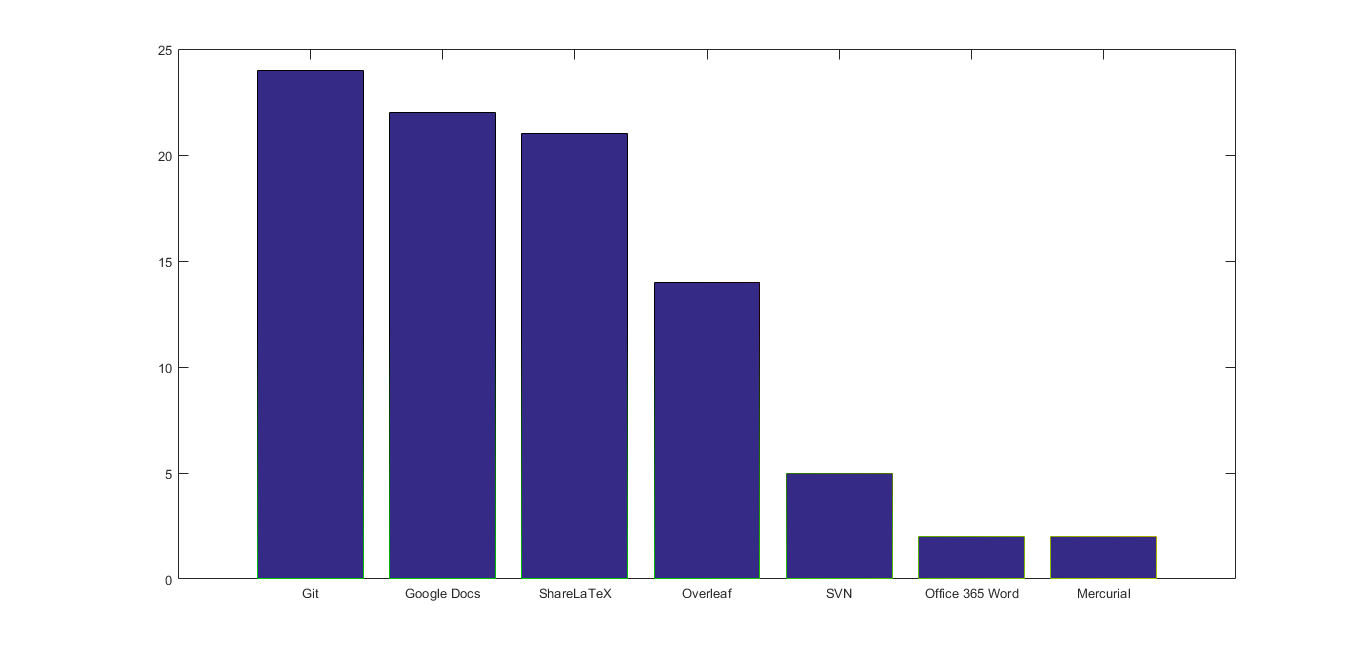
\includegraphics[width=150mm,height=75mm]{figures/best_document_tool.png}
	\caption{Visar resultatet från vilka verktyg som deltagarna tycker är bra för större dokument.}
	\label{fig:best_document_tool}
\end{figure}

\subsection{Enkät 2}
Resultaten från den andra enkäten, den om vilka erfarenheter gruppen kan ta med sig ifrån det här projektet visas nedan. Om mer detaljerade resultat önskas, se bilaga \ref{appendix:svar_enkat_dokument_erfarenheter}. Totalt var det 6 personer som svarade på enkäten.\\
\textbf{Överlag hur tycker du att hanteringen av större dokument har gått i gruppen?}\\
Fem av sex personer tycker att hanteringen av större dokument har gått bra, och en av dem tycker att det gått väldigt bra. En person tycker att det gått helt okej men kunde varit bättre.\\\\
\textbf{Vilket verktyg tycker du har varit bäst att använda?}\\
En person har ingen åsikt på frågan och en annan person tycker att båda verktygen varit lika bra att använda för större dokument. Fyra personer tycker att kombinationen \latex och Git var det bästa att använda.\\\\
\textbf{Varför tycker du det?}\\
Personen som inte har någon åsikt i frågan och den som tyckte att båda alternativen var bra, tycker inga av alternativen har varit bäst, båda verktygen hade sina egna problem. \latex och Git fungerade smidigare, hade versionshantering, historik och vem som skrivit vad, är de bra delarna av de som tyckte att \latex och Git var bättre att använda.\\\\
\textbf{För kandidatrapporten, tycker du att det var bättre med separata filer än en gemensam fil?}\\
Alla deltagare i enkäten tyckte att separata filer var bättre att använda än en stor gemensam fil för kandidatrapporten.

\section{Diskussion}
\label{sec:discussion-tuhkala}
Nedan kommer min diskussion om resultaten jag fått. De är indelade efter frågeställningarna.

\subsection{Vilka fördelar och nackdelar finns det med att använda \latex eller Word när man skriver dokument?}
Att \latex-användare var långsammare att skriva dokument än Word-användare tycker jag inte är jättemärkligt, eftersom att de som använder \latex skriver mer än de som skriver Word. Detta för att \latex-användarna måste skriva kommandon för att åstadkomma en viss sak medan Word-användare behöver bara använda sig av WYSIWYG-editor som finns inbyggd i Word där man klickar på knappar och drar tabeller i dokumentet. Word-användare använder också ett anpassat program för att skriva dokument, likt en IDE för programmering. \latex har inte lika många anpassade editorer som Word, utan där kompilerar man dokumenten istället och skriver texten i någon annan editor som vanligtvis inte har stöd för \latex kommandon.

Från resultatet ser vi också att inlärningskurvan för Word inte är väldigt stor och kräver inte mycket av användaren för att förstå och använda programmet. Det håller jag med om eftersom man behöver inte lära sig kommandon, hur man kompilerar och hur man sätter upp sin \latex-miljö. I Word får man ett program som är en WYSIWYG-editor, där man för det mesta skriver texten man vill få fram.

Det Henrik Henriksson tog upp i sin rapport om att ha en standardisering på \latex dokument skulle ha gjort att våra dokument såg likadant ut överallt. Det hade varit bättre, för till exempel när vi använde Overleaf var det några som använda mellanslag för indentering och andra som använde tabbar för det. För en del av medlemmarna i gruppen var det första gången de använda \latex och det hade kunnat vara lättare för dem om man hade en standardisering och instruktioner för hur \latex fungerar. Att använda en linter hade också hjälpt att hitta fel i dokumentet fortare än att behöva kompilera och få kompileringsfel. Overleaf hade ingen linter vilket hade gjort det svårt att införa det där, men det finns som sagt alternativ till det.

\subsection{Vilka verktyg lämpar sig för att skriva större dokument?}
Att alla grupper som använder sig av asynkrona verktyg använder Git förvånar mig inte, just eftersom det är ett bra verktyg för att versionshantera dokument och källkod bland annat. Jag förväntade mig dock att någon grupp använde SVN eller Mercurial. De som använt sig av Git har varit väldigt nöjda och gett ett medelvärde på 4,5 på en skala från 1 till 5 på hur nöjda de varit tycker jag låter rimligt, för att det är ett väldigt bra verktyg. Eftersom jag tog ett par snarlika alternativ som till exempel Git, SVN och Mercurial samt ShareLaTeX och Overleaf där funktionaliteten inte skiljer sig så mycket åt kanske det hade varit bättre att bara fråga mer generellt om asynkrona verktyg är bättre att använda än synkrona verktyg.

För synkrona verktyg skiljer medelvärdet med 0,7 till 3,8 än för 4,5 för asynkrona. Det är också väldigt bra och jag tycker också det är bra att kunna ändra på dokument samtidigt i Overleaf och Google Docs. Majoriteten vill inte byta synkrona verktyg eller byta till ett asynkront. Det tror jag kan bero på att de inte testat att använda sig av ett asynkront verktyg tidigare för dokument.

På den sista frågan i resultatet finns det flera alternativ som ligger i topp: Git, Google Docs, ShareLaTeX och Overleaf. Ett av dem är asynkront och resten är synkrona. Jag har själv använt alla förutom ShareLaTeX fast jag tror inte det skiljer sig mycket med Overleaf, och jag tycker att alla är väldigt bra att använda för att skapa stora dokument. Om det fanns ett verktyg som kunde kombinera versionshantering med att skriva samtidigt i samma dokument tror jag det skulle ha varit bättre att använda. Detta för att man får allt i båda världar: Versionshantering och historik samt att kunna skriva samtidigt. Hur det skulle fungera vet jag dock inte.

En del av alternativen jag hade till frågorna hade inte valts alls, och jag hade inget som frågade varför man inte valde dem. Det kan ju ha varit för att man inte visste vad verktyget var för något, till exempel för Mercurial. Det kan också vara för att de inte visste vad skillnaden var mellan verktygen, om man till exempel bara använt ett av dem. Det kan också ha varit för att de inte tyckt att det var något bra alternativ alls. Det är svårt att veta utan att ha frågat om det. 

\subsection{Vilka erfarenheter kan tas med ifrån det här projektet gällande framställning av större dokument?}
Att majoriteten tycker att sättet vi arbetade med kandidatrapporten jämfört med de andra stora dokument är bättre håller jag med om. Det var enklare att ha versionshantering och historik, för att man kunde se vad som ändrades eller lades till vid varje version och vem som utförde det. Man kan gå tillbaka till en tidigare version med ett enkelt kommando. Detta kunde vi inte göra när vi använde Overleaf. Fördelen med det var att alla kunde skriva samtidigt och man inte behövde installera någon mjukvara för det. Det jag tycker var mindre bra med Git och \latex var att stycken oftast skrevs som en rad vilket ger många konflikter när man försöker sammanfoga varandras delar om man ändrat något, stort eller litet.

\subsection{Metod}
Litteraturstudien för frågeställning 1 kunde kanske ha gett ett annat eller mer utförligare svar om fler artiklar, bloggar och liknande hittats. Nu när det är rätt så få källor som jag hittat kan det ge en missrepresentativ bild av det.

Enkätundersökningen som gjordes för den andra frågeställningen kunde ha gjorts mer utförligare, genom att ställa bättre frågor eller fråga om mer utförligare svar. Till exempel "Rangordna de olika alternativen från det du hade helst använt till det du helst inte velat använda." istället för att endast bara fråga om "Vilka alternativ hade du använt i framtiden för större dokument?". Om fler personer hade svarat på den första enkäten kunde det ha gett en bättre bild på hur det ser ut. Om man låtit deltagarna testat de olika verktygen innan enkäten hade det nog gett ett bättre resultat. Jag tror inte att de flesta som gjorde enkäten testat alla alternativ utan möjligtvis två stycken.

Urvalsgruppen är alla projektgrupper som läser kandidatprojektet och det kanske inte ger en representativ generell bild av arbete på större dokument än om urvalsgruppen innehållit andra yrken eller liknande. Vissa av alternativen kan förekomma mer inom företag än andra ställen.

Den andra enkätundersökningen kunde ha haft en till fråga "Vad var det som var dåligt med hanteringen av större dokument?". Som det ser ut nu får man bara de bra sakerna med verktygen. Kunde också ha frågat om det finns något annat verktyg än de vi använde som kunde ha varit bättre. Att använda sig av en enkät för att ta reda på vad gruppmedlemmar tycker kan både vara bra och dåligt. Det dåliga är att det bara är mina frågor som kommer fram medan andra frågor kan komma upp om man intervjuar istället. Det blir lite skillnad på en enkät och en intervju. Det som är bra är att det går fort att göra och att det är enklare att sammanställa svaren.

\subsection{Källkritik}

\section{Slutsatser}
\label{sec:conclusions-tuhkala}
Nedan visas slutsatserna som kommit fram från resultatet för de tre frågeställningarna:

\subsection{Vilka fördelar och nackdelar finns det med att använda \latex eller Word när man skriver dokument?}
Det jag fått fram genom min litteraturstudie är att båda alternativen har fördelar och nackdelar samt att det inte skiljer sig mycket mellan dem. Word-användare skriver dokument snabbare än vad \latex-användare gör. Inlärningskurvan är inte särskilt stor för att lära sig och använda Word. För att skriva större matematiska texter är det ingen skillnad mellan alternativen eftersom båda gör det med hög kvalitet. Att ha en standardisering och utbildning i \latex kan hjälpa nybörjare.

\subsection{Vilka verktyg lämpar sig för att skriva större dokument?}
Det jag kommit fram till med hjälp av min enkätundersökning är att Git, Google Docs och ShareLaTeX kan vara bra verktyg att använda sig av när man skriver större dokument. Overleaf kan också vara ett bra verktyg att använda sig av. Mindre lämpliga verktyg att använda är SVN, Office 365 Word och Mercurial. De verktyg som dem använde i gruppen är de väldigt nöjda med.

\subsection{Vilka erfarenheter kan tas med ifrån det här projektet gällande framställning av större dokument?}
De erfarenheter som kan tas med ifrån detta projekt är att \latex och Git har varit det bästa verktyget att använda vid framställning av större dokument. \latex och Overleaf har också varit bra men fördelarna med Git har övervägt det. Separation av dokumentet i flera mindre filer har också varit bättre än att ha en stor gemensam fil.

%%%%%%%%%%%%%%%%%%%%%%%%%%%%%%%%%%%%%%%%%%%%%%%%%%%%%%%%%%%%%%%%%%%%%%
%%% tuhkala-report.tex ends here

\chapter{Kvalitetsarbete i praktiken}
\label{cha:indiv-report-wallstrom}
\chapterprecis{\LARGE{---- Fredrik Wallström ----}}


\section{Inledning}
\label{sec:introduction-wallstrom}

De flesta företag ute på marknaden idag strävar mot att utveckla bättre produkter, vassare tjänster och smidigare processer. Dessa produkter, tjänster och processer blir alltmer komplexa, samtidigt som företagen strävar efter att bli alltmer kostnadseffektiva. I arbetet med att utveckla nya produkter spelar kvalitetsarbetet en betydande roll. Det är ett problem att effektivisera kvalitetsarbetet för att hinna med dagens utveckling, då inte ens konsumenterna själva hinner med. Kvalitetssäkring är generellt ett komplext ämne att behandla, på grund av dess diffusa definition men det står klart att det är en viktig komponent i utvecklingen av dagens produkter, tjänster och processer.

\subsection{Syfte}
\label{sec:purpose-wallstrom}

Syftet med denna rapport är att ta reda på vad det innebär att kvalitetssäkra ett mjukvarusystem och vilka metoder det finns för ändamålet. Syftet är också att se över hur kvalitetsarbetet används i praktiken, samt om det finns möjligheter att utveckla och effektivisera detta arbete. Detta undersöks eftersom det blir alltmer aktuellt på grund av den snabba utvecklingen av produkter, tjänster och processer bland företagen i dagens samhälle.

\subsection{Frågeställning}
\label{sec:issue-wallstrom}

De frågeställningar som denna rapport kommer ta upp är:

\begin{enumerate}
	\item Vad är effekterna av att kvalitetssäkra mjukvaran för en produkt med den specifika metoden kodgranskning?
	\item Vad är de egentliga kostnaderna med att kvalitetssäkra en produkts mjukvara med kodgranskning, kommer effekterna för kvalitetssäkringen kompensera för den faktiska tidsåtgången?
\end{enumerate}

\clearpage

\section{Bakgrund}
\label{sec:background-wallstrom}

Kodgranskning är en vanlig process för att öka kvaliten på koden och för att utsända kunskap inom projektet där koden är aktiv. Den här studien har genomförts för att se vilken påverkan en modern kodgranskningsprocess har på kvaliten hos ett mjukvarusystem. 

Studien har också undersökt vad det är som gör att kodgranskning har blivit en viktig del för att kvalitetssäkra ett mjukvarusystem och vad de praktiska fördelarna är med en modern kodgranskningsprocess. Det är alltså intressant att se vilka problem som löses med hjälp av denna process. 

\section{Teori}
\label{sec:theory-wallstrom}
Nedan följer information om de ämnen som behandlas i rapporten. Informationen beskriver vad kvalitetssäkring innebär, vad kodgranskning är för något och hur det specifika kodgranskningsverktyget Gerrit fungerar.

\subsection{Kvalitetssäkring}
Att säkerställa hög kvalité på ett system idag, innebär inte bara att testa och analysera systemet att det fungerar korrekt. För att försäkra sig själv och framförallt övertyga användaren om att systemet är i bra skick och presterar väl, kräver hög nogrannhet och disciplinerat kvalitetsarbete. Kvalitetssäkran är en process som genomförs kontinuerligt under uppbyggnaden av ett system och ingenting som appliceras vid systemet slutfas \cite{feldman2005quality}.

Att genomföra en kvalitetssäkrande process innebär enligt definiton, att tillhandahålla en försäkran om att programvaruprodukten och processer i produktens livscykel överensstämmer med deras specifika krav och håller fast vid de uppsatta planerna. \textit{Process}, är nyckelordet för kvalitetssäkran, det innebär alltså att kvalitetssäkran är en metod och inte en enstaka teknik. En annan viktig aspekt för kvalitetssäkran är att det inte behandlas som ett filosofiskt problem, utan mer som ett mätbart problem. Slutligen innebär kvalitetssäkran om att ge garantier och trovärdighet, produkten ska fungera rätt och folk ska tro att den fungerar rätt \cite{feldman2005quality}.

Kvalitetssäkran innefattar \textit{testning} som en av de viktigare aktiviteterna. Det finns dock ett ordspråk som säger att det inte går att testa kvaliten i produkten, utan att en testplan enbart kan fånga fel och ge ett mått på kvaliten. Det finns olika kvalitetssäkrande processer, de definieras för att passa behoven hos produkten. En process kan definieras för att försäkra sig om att designen är lämplig, implementationen är nogrann och att produkten möter alla krav innan publicering. Denna process kan även utvecklas till att analysera de upptäckta defekterna och sedan ständigt förbättra dessa \cite{feldman2005quality}.


\subsection{Kodgranskning}
Kodgranskning uppfattas som en effektiv process för att upptäcka fel och och fixa systemets defekter innan koden integreras med kodbasen \cite{mcintosh2014impact}. Denna process definierades av Fagan \cite{fagan1999design} och innebär att granskarna ska metodiskt följa checklistor för att sedan medverka i gruppmöten tillsammans med kodens författare. Kodgranskning har under åren moderniserats till att bli en flexibel lättviktsvariant av Fagans tidiga process. En modern kodgranskning består inte av checklistor eller personliga möten, utan den sker online. Idag finns det verktyg att ta hjälp av vid kodgranskning, bland annat har kodgranskning blivit starkt integrerat i olika versionshanteringsverktyg och problemhanteringssystem. Gerrit är ett exempel på ett väl använt och utvecklat verktyg för att underlätta kodgranskningsprocessen. Det finns alltså mycket som skiljer den moderna kodgranskningsprocessen med den som tillämpades förr, de båda har dock samma syfte, vilket är är att förbättra kvaliten på systemet \cite{shimagaki2016study}. 

Den generella processen för en modern kodgranskning kan sammafattas som följer. Först gör en utvecklare en ändring i koden och överlämnar den för granskning. I andra steget diskuterar andra utvecklare ändringarna och föreslår eventuella förbättringar i koden. Till sist accepterar en eller flera granskare ändringarna och koden integreras med kodbasen \cite{kitagawa2016code}.

\subsection{Gerrit}
Gerrit är ett modernt kodgranskningsverktyg som underlättar en kodgranskningsprocess för ett projekt som använder git för versionshantering. Gerrit integrerar automatisk med testverktyg samt med kodverktyg. Metoden som används för att använda Gerrit är att författaren av koden laddar upp förslag på ändringar i systemet till en Gerrit server. Sedan kommer recensenter att evaluera koden och ge förslag på eventuella förbättringar. För att koden sedan ska godkännas kommer en kontrollant evaluera koden och verifiera dess korrekthet. Detta låter som en vanlig modern kodgranskningprocess men det som Gerrit underlättar med är det grafiska gränsnittet. Det hjälper till att få en överblick över statusen för de förslagna ändringarna. Gerrit ger också en möjlighet för teams att sätta olika krav och bekräftelse kriterier som krävs innan den förslagna ändringen integreras med kodbasen \cite{mcintosh2014impact}.

\section{Metod}
\label{sec:method-wallstrom}

För att förstå effekterna av att genomföra en kodgranskningsprocess samt att inse vad de egentliga kostnaderna är med att kvalitetssäkra en produkt har en kvalitativ litteraturstudie genomförts. Litteraturstudien bestod av att analysera och bearbeta olika vetenskapliga rapporter som var relevant för ämnet ifråga. De utvalda rapporterna hade genomfört intressanta experiment och utredningar som kändes trovärdiga.

För att undersöka dessa frågor med en koppling till praktiken så har även ett praktiskt experiment gjorts på studenter ifrån Linköpings universitet. Dessa studenter har genomfört ett projekt där fokus var att leverera ett färdigt system med hög kvalité till kund. Experimentet bestod av att studenterna skulle svara på en enkät om hur det är att jobba med en kvalitetssäkrande process. Frågorna som studenterna fick svara på var följande:

\begin{itemize}
	\item Hur anser du det är att jobba med en kvalitetssäkrande process, är det positivt eller negativt, om man tar den faktiska tidsåtgången i åtanke?
	\item Har du jobbat med den specifika metoden kodgranskning för att säkerställa kvaliten på en produkt?
	\item Tycker du att kodgranskning hjälper att kvalitetssäkra en produkt?
	\item Anser du graden av deltagande människor i kodgranskningen hjälper eller försämrar kvaliten hos produkten? Blir det för komplicerat att anordna möten, tidsåtgången blir för stor, det tar för lång tid att få koden godkänd med mera.
	\item Har du några övriga tankar om att arbeta med en kvalitetssäkrande process eller med kodgranskning?
\end{itemize}

Detta experiment valdes eftersom att enbart utgå ifrån litteraturstudier inte ger en representativ bild av de relevanta kvalitetsfrågorna. Experimentets syfte var att se hur kvalitetsarbete fungerar i praktiken. Det är också intressant att se hur detta experiment skiljer sig ifrån resultatet av litteraturstudien. Det valdes studenter från Linköpings universitet eftersom det var viktigt att studenterna har jobbat med en kvalitetssäkrande process, vilket de har gjort under deras kandidatarbete.

\section{Resultat}
\label{sec:results-wallstrom}
Nedan följer resultatet ifrån den litteraturstudie som genomförts och ifrån den enkät som genomfördes på studenter ifrån Linköpings universitet. 

\subsection{Litteraturstudie}
McIntosh \cite{mcintosh2014impact} visar med en empirisk studie vilken påverkan en modern kodgranskningsprocess har på kvaliten hos ett mjukvarusystem. McIntosh analyserar huruvida det finns en relation mellan kodgranskning och kvalité genom att studera 3 stycken projekt. Dessa projekt drivs av en kodgranskningsprocess som använder sig av verktyget Gerrit. Studierna går ut på att undersöka hur kvaliten påverkas beroende på hur stor del av koden som har blivit kodgranskad och hur många recensenter som deltagit i kodgranskningen. Det visar sig att både andelen kod granskad och hur många som har deltagit i kodgranskningen har en koppling till kvalité. Låg andel kod granskad samt lågt deltagande visar sig skapa mellan 2 till 5 stycken extra defekter efter produktlansering. McIntosh bekräftar med sin empiriska studie att dåligt granskad kod har negativa effekter på kvaliten hos ett mjukvarusystem.

Beller \cite{beller2014modern} visar med en empirisk studie vad de praktiska fördelarna är med en modern kodgranskningsprocess. Studien går ut på att manuellt klassificera 1400 ändringar som gjorts i en kodgranskningsprocess för öppen källkod. Beller kommer fram till att 7-35\% av de granskade kommentarerna kasseras samt att 10-22\% av ändringarna inte utlöstes av en kommentar ifrån kodgranskningen. Bellers slutsats är även att en homogen kodgranskning leder till samma antal ändringar i koden, oberoende på granskaren. Det är alltså typen av uppgifter som spelar roll, mindre uppgifter ger upphov till mindre ändringar och större uppgifter som involverar större kodkärna samt fler filer, leder till fler ändringar.

\subsection{Enkät}
De sammanfattade resultaten ifrån den genomförda enkäten presenteras nedan, för mer detaljerade resultat, se bilaga \ref{appendix:svar_enkat_kvalitet}.
\begin{itemize}
	\item \textbf{100\%} anser att det är positivt att jobba med en kvalitetsäkrande process.
	\item \textbf{88\%} har jobbat med den specifika metoden kodgranskningen för att säkerställa kvaliten hos en produkt.
	\item \textbf{100\%} anser att kodgranskning hjälper till att kvalitetssäkra en produkt.
\end{itemize}
Figur \ref{fig:grade_participation} nedan visar resultatet från frågan om graden av deltagande människor i en kodgranskningsprocess hjälper eller försämrar kvaliten hos en produkt.

\begin{figure}[H]
	\centering
	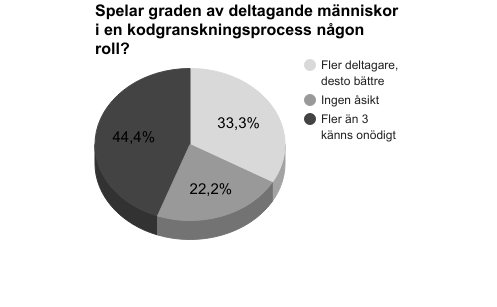
\includegraphics[width=100mm]{figures/grade_participation.png}
	\caption{Visar resultatet från om graden av deltagande människor i en kodgransningsprocess spelar någon roll.}
	\label{fig:grade_participation}
\end{figure}

\section{Diskussion}
\label{sec:discussion-wallstrom}
Resultatet av den genomförda enkäten visar att effekterna av en kodgranskningsprocess är positiva. 100\% anser att kodgranskning hjälper till att kvalitetssäkra en produkt. Det är endast få personer som inte använt sig av den specifika metoden kodgranskning för att kvalitetssäkra en produkt, utan istället använt sig av pargprogrammering. Den här datan är inte tillräcklig och är en avgränsning i denna studie, för en mer representativ bild skulle det krävas större mängd data. 

Det intressanta med resultatet ifrån enkäten är att 44,4\% av de som deltog anser att om fler än 3 personer deltar i en kodgranskningsprocess finns det risk att tidsåtgången inte kompenserar för den faktiska vinsten med granskningen. Detta är också något som Beller \cite{beller2014modern} kommer fram till i sin studie angående vilka problem som löses med hjälp av kodgranskning. Beller anser att en homogen kodgranskning leder till samma antalet ändringar i koden, oberoende av vem som granskar. Det spelar alltså inte någon roll vem som granskar koden, den kommer heller inte blir bättre desto fler som granskar. Resultatet tyder alltså på att en kodgranskningsprocess inte bör innehålla fler deltagande personer än tre för att kvalitetssäkra produkten. 

Samtidigt visar McIntosh \cite{mcintosh2014impact} att kodgranskningsprocesser med lågt deltagande uppskattningsvis innehåller upp till 5 stycken defekter efter lansering, vilket kan låta som en kontradiktion till Bellers \cite{beller2014modern} resultat. McIntosh specificerar dock inte att det finns ett optimalt antal personer som ska delta i en kodgranskningsprocess för att göra den så effektiv och kvalitetssäkrande som möjligt. Den intressanta fråga som jag då ställer mig är om det finns ett optimalt antal deltagande personer i en kodgranskningsprocess? Det är en fråga som utifrån egna slutsatser inte finns något svar på. Det är en bred fråga och beror på hur stort projektet är och vad det finns för kvalitetsmål på produkten. Desto högre kvalitetsmål, desto fler personer bör delta i kodgranskningsprocesserna känns intuitivt som en bra approach. Denna studie visar dock att så inte är fallet, kodgranskningen riskerar att bli ineffektiv vilket således kan leda till en icke komplett produkt. Det här är en intressant frågeställning som kräver vidare efterforskning. Även här finns det såklart avgränsningar som bör tas med i åtanke. Dels innehåller inte enkäten tillräckligt med data och därtill skulle det även behövas göra en mer omfattande litteraturstudie för att få en representativ bild över situationen.

 

\section{Slutsatser}
\label{sec:conclusions-wallstrom}
Utifrån den genomförda enkäten men framförallt utifrån den gjorda litteratustudien visar denna rapport att kvalité och kodgranskning har en stark relation. Att genomföra en kodgranskningsprocess visar sig tydligt ha positiva effekter på produktens kvalité. För att svara på fråga 1 i \ref{sec:issue-wallstrom} så tyder resultatet från denna studie på att effekterna av en kodgranskningsprocess är positiva ur kvalitetssynpunkt. McIntosh \cite{mcintosh2014impact} visar att en dåligt granskad kod ger upphov till 2-5 stycken extra defekter efter produktlansering.

För att svara på fråga 2 i \ref{sec:issue-wallstrom} så tyder resultatet från denna studie att kostnaden för en kodgranskningsprocess kompenserar för den faktiska tidsåtgången. Den genomförda enkäten visade att 100\% av deltagarna anser att kodgranskning hjälper till att kvalitetssäkra en produkt. Enkäten visar också att graden av deltagande människor i kodgranskningen inte behöver överstiga 3 stycken, detta kan leda till onödig tidsåtgång. Det här är även något som bekräftas av Bellers studie \cite{beller2014modern}. Slutsatsen av detta är att effekterna av en kodgranskningsprocess kompeserar den faktiska tidsåtgången så länge antalet personer som granskar inte överstiger 3 stycken.


%%%%%%%%%%%%%%%%%%%%%%%%%%%%%%%%%%%%%%%%%%%%%%%%%%%%%%%%%%%%%%%%%%%%%%
%%% person-report.tex ends here

\printbibliography

\end{document}

%%%%%%%%%%%%%%%%%%%%%%%%%%%%%%%%%%%%%%%%%%%%%%%%%%%%%%%%%%%%%%%%%%%%%%
%%% student_thesis.tex ends here